%\documentclass[openany,titlepage,12pt,post]{octavo}
%foolscap,crown, post, largepost, 
%demy, medium, royal, superroyal and imperial
\documentclass[openany,titlepage,12pt]{book}
\usepackage{geometry}
\geometry{
    a5paper,
    total={67mm,137mm}%,
    %total={67mm,134mm}%,
    %left=2mm,
    %top=20mm,
}

\usepackage[utf8]{inputenc}
\usepackage{fontspec}
\usepackage{graphicx}
\graphicspath{ {../images/} }

\usepackage{fontspec}
\usepackage{lettrine}
\usepackage{Typocaps}
\usepackage{Zallman}
\usepackage{ragged2e}
\usepackage{changepage}

\usepackage[portuguese]{babel}
\usepackage{hyphenat}
\hyphenation{mate-mática recu-perar}

\usepackage{fwlw}
\usepackage{fancyhdr}
\pagestyle{fancy}
\fancyhead[CO]{\textit{\rightmark}}
\fancyhead[CE]{\textit{\leftmark}}
\fancyhead[LO]{\thepage}
\fancyhead[RE]{\thepage}
\fancyhead[LE,RO]{}
\fancyfoot[L,C]{}
\fancyfoot[R]{\usebox\NextWordBox}
\renewcommand{\headrulewidth}{0pt}
\renewcommand{\footrulewidth}{0pt}

\fancypagestyle{plain}{
  \fancyhead{}
  \fancyhead[LO,RE]{\thepage}
  \fancyfoot[C]{}%{\thepage}%
  \fancyfoot[R]{\usebox\NextWordBox}
  \renewcommand{\headrulewidth}{0pt}% Line at the header invisible
  \renewcommand{\footrulewidth}{0pt}% Line at the footer visible
}

\renewcommand{\chaptermark}[1]{\markboth{#1}{}}
\renewcommand{\sectionmark}[1]{\gdef\rightmark{#1}}
%\renewcommand{\sectionmark}[1]{\markright{\arabic{section}.\ #1}}

\usepackage{titlesec}%{}{}{0em}{\bf\LARGE}
\titleformat{\chapter}[display]
  {\normalfont\Large\centering}
  {\centering }%\thechapter}%\chaptertitlename
  {0pt}
  {}%{\Large}
\titlespacing*{\chapter} 
  {0pt}
  {6pt}
  {6pt}

\titleformat{\section}
  {\centering\normalfont
  \fontsize{13}{14} \selectfont}
  %{\thesection}
  {}{1em}{}
\titlespacing*{\section} 
   {0pt}
   {12pt}
   {12pt}
 
\titleformat{\subsection}
   {\centering\normalfont\normalsize\itshape}
   {}{1em}{}
\titlespacing*{\subsection} 
    {0pt}
    {10pt}
    {10pt}

\title{CATECISMO BRASILICO}
\author{Araújo}
\date{1686}

\newcommand{\lgS}{\char"017F}
\newcommand{\lgSS}{\char"017F\char"017F}

\usepackage{enumitem}
\setlist[enumerate]{
    leftmargin=6pt,
    topsep=3pt,
    parsep=-5pt,
    partopsep=0pt,
    itemindent=6pt
}
% \setlist[enumerate]{
%     leftmargin=12pt,
%     topsep=3pt,
%     parsep=-5pt,
%     partopsep=0pt,
%     labelsep=4pt,
%     itemindent=4pt,
%     itemsep=4pt
% }

\usepackage{etoolbox}
\newlist{alternate}{enumerate}{1}
\renewcommand\labelalternatei{\protect\ifnumodd{\value{alternatei}}{M.}{D.}}
\setlist[alternate]{
    leftmargin=6pt,
    topsep=3pt,
    parsep=-5pt,
    partopsep=0pt,
    itemindent=6pt
}
\newlist{altereven}{enumerate}{1}
\renewcommand\labelaltereveni{\protect\ifnumodd{\value{altereveni}}{D.}{M.}}
\setlist[altereven]{
    leftmargin=6pt,
    topsep=3pt,
    parsep=-5pt,
    partopsep=0pt,
    itemindent=6pt
}

\newcommand{\comecalista}[5]{
    \hspace*{-11.7pt}
    \begin{minipage}[t]{0.08\linewidth}
        \flushright #1\\#2
    \end{minipage}
    \hspace{0pt}
    \begin{minipage}[t]{0.94\linewidth}
        \lettrine
        [findent =2pt, nindent=0pt,  lines=2]
        {#3}{#4}#5
    \end{minipage}
    \vspace*{-3pt}
}

\begin{document}

%\setmainfont[Ligatures=Historic, Style=Historic]
\setmainfont[Ligatures=Historic]
% %{Liberation Serif}%
% %{DejaVu Serif}%
{EB Garamond}
\maketitle

\begin{titlepage}
    \begin{center}
        CATECISMO
        \vspace*{15pt}

        {\huge BRASILICO}
        \vspace*{15pt}

        {\tiny DA}
        \vspace*{15pt}

        DOUTRINA CHRISTAÃ
        \vspace*{15pt}

        {\tiny PUBLICADO DE NOVO} 
        \vspace*{15pt}

        {\tiny POR}
        \vspace*{15pt}

        JULIO PLATZMANN
        \vspace*{15pt}

        {\tiny EDIÇÂO FACSIMILAR}
        \vspace*{60pt}

        {\tiny LEIPZIG
        \vspace*{15pt}

        B. G. TEUBNER
        \vspace*{15pt}

        1898}

    \end{center}  
    \clearpage
\end{titlepage}

\begin{center}
    \vspace*{20pt}
    {\huge CATECISMO}
    \vspace*{20pt}

    {\large BRASILICO}
\end{center}
\pagebreak

%começa o texto
\begin{center}
    {\large CATECISMO\\}
    \vspace*{8pt}
    {\huge BRASILICO}
    \textit{\\Da Doutrina Chri\lgS tãa,}
    \\Com o Ceremonial dos Sacramentos, \&
    \\mais actos Parochiaes.
    \textit{\\COMPOSTO}
    \\Por Padres Doutos da Companhia de
    \\JESUS,
    \textit{\\Aperfeiçoado, \& dado a luz}
    \\Pelo Padre ANTONIO DE ARAUJO
    \\da me\lgS ma Companhia,
    \textit{\\Emendado ne\lgS ta \lgS egunda impre\lgSS aõ}
    \\Pelo P.BERTHOLAMEU DE LEAM
    \\da me\lgS ma Companhia,

    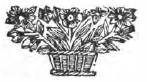
\includegraphics{img}
    \\{\huge LISBOA.}
    \\Na Officina de MIGUEL DESLANDES
    \\M. D C. L X X X V I
    \textit{\\Com todas as licenças nece\lgSS arias}

\end{center}
\clearpage
\pagebreak
%Começo do primeiro capítulo
%\vspace*{-\baselineskip}
\begin{center}
    
\includegraphics[scale=0.20]{01-poemas_brasilicos.png}
\end{center}
\unskip
\vspace*{-20pt}
{\let\clearpage\relax \chapter{POEMAS BRASILICOS}}%\chapter{POEMAS BRASILICOS}
\chaptermark{Poemas Bra\lgS ilicos}
\vspace{10pt}

\section{Do Padre Chri\lgS tovaõ Valente,\\Theologo da Companhia de JESUS,}
\sectionmark{Poemas Bra\lgS ilicos}

\subsection{Emendados para os mininos cantarem\\
ao Santi\lgSS imo nome de JESUS.}

\lettrine[findent =4pt, nindent=0pt, lines=5]
{\zall{I}}{E}SU, moropyçyroána,\\
JESU, tecó catú iâra,\\
JESU, toryberecoára,\\
JESU, xe poçánga ymána\\
JESU, xe remimotára.

Päí JESU, xepoçánga,\\
Xe pyá, xe recobé,\\
Xe pëá umé iepé,\\
Eporauçuboc xe ánga,\\
Tipyatã nde recé.

Nde po guyripe xe nónga\\
Nde morerecoár xe ri,\\
Toçó xe ánga iepí\\
Tecó catú monõonga\\%nova página
Nde rakypoéra rupí.

Xe pyá, xe ánga eiár\\
Nde mbäéramo tauié:\\
Xe möapyçyc iepé,\\
Nde rausûba aipotár\\
Cauçubipyra çocé.

Ocykyié nde çüí\\
Anhánga nde möabáetêbo\\
Eiorí emoçykyiêbo,\\
Toçó umé ôca rupí\\
Oré ânga monghüêbo.

Nde popé eré ânga rui,\\
Oré rerecoâreté:\\
Oroierobiá nde recé,\\
Oré recobé pucuí\\
Oré rauçubá iepé.

\subsection{A Virgem Santi\lgSS ima Maria Mãy de Deos Senhora No\lgSS a.}

\begin{center}
    MOTE.
\end{center}
\unskip
\vspace{\baselineskip}
\lettrine[findent =4pt, nindent=0pt, lines=2]
{T}{U}pã çy angaturáma,\\
Santa Maria xe iára,\\
Nde reçá porauçubára\\
Xe recó catúãoáma\\
Xe ánga remïecára\\
GLOSSA.%nova página
%\vspace{\baselineskip}
\lettrine[findent =4pt, nindent=0pt, lines=2]
{A}{B}abycagoérëyma,\\
Caräíbebé poaitâra,\\
Ybácpôra mborypâra,\\
Tecótebẽçâbëyma,\\
Anhânga momocembâra.

Enëĩ morerecoâra,\\
Icó xe nhëéng päâma,\\
JESUS robaké möâma,\\
Tecó catú angagoâra,\\
Tupã cy angaturama.

Ereicatú xe pëâbo\\
Anhánga recó süí:\\
Xe catú âoâma ri\\
Enëĩ xemboguatâbo\\
Nde angaturama rupí.

Xe iekyîme bé corí.\\
Emocanhem xe räangâra:\\
Xe ánga nde rauçupâra\\
Eraçó ceroieupí,\\
Santa Maria xe iâra.

Abápe nde renoîdâra\\
Oçó tenhé nde çüí?\\
Enhemoçainan xe rí:\\
Moreauçûba rerecoâra\\
Nde rerapoâna iepí.%nova página

Ybypôra aipó ëí;\\
Cëyinhê nde recaçâra,\\
Apyâba abé mombegoâra.\\
Oimoçaĩ tába rupí\\
Nde reçá porauçubâra.

Otĩ coaracy ocêma\\
Nde berâba robaké;\\
Iacy tatá cuêpe é\\
Inhemimi, nde cöêma\\
Ara rorypâbeté.

Apyâba dëitëé\\
Oybamo nde möâma:\\
Nëĩ, nëĩ epüâma\\
Tereimëéng opábenhé\\
Xe recó catú ãoâma.

Tupã JESUS nde membyra\\
Oimöin çupí mbäé,\\
Iangaipábäé dëitëé\\
Oceca eté nde poguyra\\
Oiecoçurëymebé.

Xe angaipabóramo abé\\
Aipouçú eté eté xe iára,\\
Iorí xe pyçyrõçâra\\
Xe moiecoçúb iepé,\\
Xe ánga remiecâra.\\%nova página
\newpage

\subsection{Ao Santo Anjo da Guarda.}
\begin{center} 
    ESTRIBILHO
\end{center}
\unskip
\vspace{\baselineskip}
\lettrine[findent =4pt, nindent=0pt, lines=2]
{P}{E}iorí apyábetá,\\
Oiepé tiaimöeté\\
Iandé Caräíbebé.

\begin{center}
    \textit{Copla.}
\end{center}

\lettrine[findent =4pt, nindent=0pt, lines=2]
{X}{E} raroâna ybakyguâra,\\
Caräíbebé porânga,\\
Eimböé catú xe ánga,\\
Toicüáb ybâca piâra.\\
Xe rúba, xe rerecoâra,\\
Nde recé nho taguatá\\
Eipëá xe räangâra,\\
Peiorí, apyábetá,\\
Oiepé tiaimöeté\\
Iandé Caräíbebé.

Tupã robaké eicôbo\\
Xe çüí derecyryki,\\
Naxemopyá typyki\\
Anhânga xerapecôbo.\\
Deitëé moxy oçôbo\\
Oätápe xe reiá\\%nova página
Nde po guyrpe xe moingôbo,\\
Peierî apyábetá, \&c.

Xe irúnamo memé\\
Nde ãme xe rauçubâbo,\\
Tecó angaipâba pupé.\\
Dotĩi cerã acé\\
Marã oicôbo ára ia.\\
Oäräâna robaké,\\
Peiorí, apyábetá, \&c.

\subsection{Do Santi\lgSS imo Sacramento da Euchari\lgS tia.}
\begin{center}
    ESTRIBILHO.
\end{center}

\lettrine[findent =4pt, nindent=0pt, lines=2]
{M}{Y}iapé ybakygoâra,\\
Apyábebé rembïú,\\
Xe ánga recó pucú.

\begin{center}
    \textit{Copla.}
\end{center}

\lettrine[findent =4pt, nindent=0pt, lines=2]
{X}{E} ambyacy poçánga,\\
Xe recó tebẽ rupiâra,\\
Ecepiác xe maräâra,\\
Tereçauçubár xe ánga.\\
Iorí xe recó monhánga,\\
Myiapé ybakygoâra,\\
Apyábebé rembïú\\%nova página
Xe ánga recó pucú.

Xe ánga taÿgäyba,\\
Xe ánga ierobiaçâba,\\
Ybypôra moeçaĩbâba,\\
Ybâca pôra roryba,\\
Moreauçubâra yba,\\
Myiapé ybakygoâra, \&c.

Nde angaturâma rí\\
Eiorí xe poreauçubôca\\
Eipytybyróc xe róca\\
Nde pytaçâba iepí,\\
Taguatá nho nde rupí,\\
Myiapé ybakygoâra, \&c.

Iangaturámbäé çupé\\
Myiapé tecobé iára:\\
Ipoxybäé taçâra\\
Tëõoguár oioupé:\\
Oiepé mbïú pupé\\
Pecepiác tecóparâba?\\
Apyábebé rembïú,\\
Xe ánga recó pucú.
\newpage

\begin{center}
    
\includegraphics[scale=0.20]{02-aos_religiosos.png}
\end{center}
\section{Aos Religiosos da Companhia de 
JESUS do E\lgS tado do Bra\lgS il.}
\chaptermark{}
\sectionmark{}
\vspace*{14pt}

\lettrine[findent=2pt, nindent=0pt, lines=2]
{S}{A}e de novo a luz o Cateci\lgS mo Bra\lgS ili-\linebreak
co, que já no anno de 1618a vio a primeira vez. E \lgS ae
com algũa variedade. Porque \lgS e trocaraõ alguns vocabulos 
daquella idade, que já hoje e\lgS tranha o commum idio-
ma dos Bra\lgS is, em outros, que \lgS aõ hoje vulgares. A e\lgS 
crita \lgS e emendou em orthogra-phia mais proporcionada á 
locuçaõ Bra\lgS ili-ca. No texto da Doutrina, \& Dialogos he
rara a alteraçaõ. Pois \lgS ó \lgS e mudáraõ algũas \lgS 
entenças, que o exercício de tantos annos notou menos 
perceptiveis: \& em \lgS eu lugar\linebreak \lgS e \lgS u\lgS  
tituiraõ outras com termos,\& palavras mais nece\lgSS arias 
á intelligencia dos my\lgS terios que aqui \lgS e inculcaõ. 
Finalmente tiraraõ\lgS e  algũas exortaçoẽs, \& praticas, que em
hum perfeito Cateci\lgS mo abundavaõ. O ze-\linebreak
lo, \& e\lgS pirito
de VV. RR. na \lgS alvaçaõ dos Bra\lgS is lhe conciliará a 
total perfeiçaõ, \& firmará com novos cravos a fortuna com 
que naceo. E \lgS e foi feliz na innumeravel me\lgSS e, que 
das barbaras Campanhas de\lgS ta Ameri-ca introdu\lgS io nos
celeiros de Chri\lgS to: como o E\lgS pirito, \& a indu\lgS
tria, que o menea, he a me\lgS ma, occa\lgS ionará \lgS em 
duvida com repe-tidas conver\lgS oẽs venturo\lgS o aumento ao
Imperio da Igreja:\& multiplicadas laureolas a Chri\lgS to
na con\lgS ervaçaõ de\lgS ta nova Chri\lgS tãdade em \lgS eu
ob\lgS equio: como atégora admirou a experiencia, \& promete
\lgS empre a re-\linebreak ligio\lgS i\lgSS ima empre\lgS a da maior 
gloria de\linebreak
Deos, a que a Companhia a\lgS pira.
\newpage

\begin{center}
    \vspace*{12pt}
    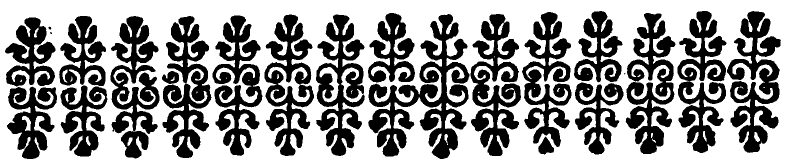
\includegraphics[scale=0.24]{03-advertencias.png}
\end{center}
\unskip
\subsection{Advertencia \lgS obre a orthographia, \&
pronunciaçaõ de\lgS te Cateci\lgS mo.}


\lettrine[findent=2pt, nindent=0pt, lines=2]
{E}{S}te Cateci\lgS mo como produ\lgS ido pelos\linebreak
Portuguezes, he Portuguez na e\lgS critu-ra; que pode admitir
a pena Portugueza.\linebreak E a\lgSS i \lgS e u\lgS a nelle de
Ç com zeura em lugar do S, cujo natural \lgS ibilo naõ con\lgS
ente a\linebreak lingoa Bra\lgS ilica. E\lgS screve\lgS e Nha,
nhe, \&c. para formar aquella voz, que \lgS e prefere nas 
ultimas \lgS yllabas de\lgS tas no\lgSS as palavras,
Tenha, Tenho.

Ne\lgS ta lingoa ha concur\lgS o de muitas vogaes em alguns
vocabulos: das quaes talvez cada hũa faz \lgS yllaba per
\lgS i, \& muitas ve\lgS es duas, \& tres concorrem em hũa
\lgS ó \lgS yllaba. Exemplo \lgS eja o verbo Aiopoai, que
\lgS ignifi-ca, ordeno a alguem que faça algũa cou\lgS a,
no qual o primeiro A, he \lgS yllaba: Io, outra: \& as tres
ultimas vogaes fazem outra \lgS ylla-ba, na qual O, he liquido,
AI, diphtongo. Para \lgS e evitar a duvida, que ne\lgS ta
parte podem padecer os menos ver\lgS ados ne\lgS ta lingoa,
\lgS e poem \lgS obre algũas vogaes dous pontos, como \lgS 
inal, que e\lgSS a vogal, que os tem-he \lgS olitaria, \&
faz \lgS yllaba per Vi \lgS eparada das outras. Donde \lgS e
\lgS egue, que havendo duas, ou mais vogaes \lgS em
e\lgSS es pontos, \lgS e devem unir em hũa \lgS ó \lgS yllaba.

\chaptermark{Advertencia.}
\sectionmark{Advertencia.}

C, pronuncia\lgS e a\lgS pero \lgS obre A, O, V,\& brando
\lgS obre E,I,Y, como ne\lgS te nome Portuguez, 
Concerto.Se tem zeura, \lgS e porfere brando \lgS obre
A,O,V, como no Portuguez.

K, caracter Grego \lgS e introdu\lgS io aqui por
nece\lgSS idade com o \lgS om a\lgS pero \lgS obre E, I, Y, que
\lgS e \lgS ente na voz Grega Kyrie, \& \lgS e deve dar a muitas
de\lgS ta lingoa, como Okena, por-ta: Xekirirĩ, estou tri\lgS te:
Okyr, chove. Qu, para exprimir e\lgSS e \lgS om ao modo Portuguez
de\lgS tas palavras Quero, Qui\lgS era, he incoveniente: porque 
além de viciar a proprieda-de do V, que ne\lgS ta lingoa he liquido
depois do Q, confunde a pronunciaçaõ de muitas diçoẽs, que \lgS e
e\lgS creverem do me\lgS mo modo, \& do me\lgS mo modo \lgS e naõ
pronunciariaõ, quaes \lgS aõ, Eboqué, eis aqui: Aquéa, aquela: 
Qué coty, para cá, em que V, he liquido. Oquena, porta, Açoquendá,
fecho, em \~{q} V. não he lique\lgS cente.

G, he a\lgS pero ferindo A, O, V, brando porém, \lgS obre E, I, Y,
como na palavra Portugueza, Gigante. Mas quando tiver H,
immediatamente junto a \lgS i, ferirá com a\lgS pere-\lgS a
E, I, por exemplos \lgS ejaõ, Ainmonghé,\linebreak meto dentro:
Namonhanghi, naõ faço.

H, nos exemplos acima naõ he a\lgS piraçaõ rigoro\lgS a, \lgS ó
communica a\lgS pere\lgS a ao G. Porém ne\lgS ta palabras Ahẽ,
homem: Ehẽ, \lgS im das mulheres, \& em algũas mais, \lgS e ha,
he a\lgS piraçaõ a\lgS pera, \& perceptivel, lançan-do o halito
com algũa violencia para fora.

I, nunca no idioma Bra\lgS ilico he taõ rigoro\lgS a con\lgS oante,
que fira a vogal como G, entre vogaes he cõ\lgS oante duplez, como
ne\lgS -te verbo, Aiar, tomo: onde o I, faz o me\lgS mo \lgS om,
que no no\lgSS o verbo, Caiar. E com e\lgSS a me\lgS ma vocalidade 
\lgS e enunciará, quando no principio da diçaõ e\lgS tiver antes de
vogal, co-mo em Ioauçûba, affeição mutua. Excep-to quando for
articulo, porque entaõ fará \lgS yllaba per \lgS i, \& para
di\lgS tinçaõ, ou elle, ou\linebreak a vogal \lgS eguinte terá
\lgS obre \lgS i dous pontos. Seguindo qualquer vogal fará 
com ella\linebreak diphtongo: \& quando naõ deva concor-rer
para diphtongo, a vogal antecedente\linebreak levará dous pontos
como \lgS eparada do I, o que \lgS e ve ne\lgS ta palavra
Päí, Senhor.

O, de\lgS pois de con\lgS oante , \& antes de A, ou E, as mais
ve\lgS es he liquida: exemplo, Tëõboéra, cadaver. Quando naõ for
liqui-da, terá \lgS obre \lgS i dous pontos, para fazer \lgS yllaba
per \lgS i, como Aimöáng, imagino. Seguindo a outra vogal, fará 
diphtongo com ella, como no futuro, ãoâma, v.g. xe çöãoä-ma, para
eu ir. Mas \lgS enaõ fizer diphtongo, como \lgS uccede em muitas
diçoẽs, terá a vogal antecedente dous pontos, para final, co-mo
\lgS e tem dito, que deve \lgS eparar\lgS e delle, como \lgS e ve
ne\lgS te vocabulo, Anhangäó, reprehendo com vituperio.

R, \lgS empre fere com brandura a vogal, como ne\lgS ta no\lgSS as
palavras Firo, Fera: ou e\lgS teja no principio ou no meyo da diçaõ.

V, nunca he con\lgS oante, \lgS alvo quando por melindre \lgS e 
u\lgS a no lugar de B, como por, Abá, Peçoa, Avá. Mas quando
concor-rem dous VV, \lgS obre outra vogal, fica liquido o 
\lgS egundo V, \& o primeiro parece con\lgS oan-te, porém com
\lgS om taõ brando, que \lgS oa co-mo G, exemplo, Uuîme, ahi, que
\lgS oa como Guime. De\lgS pois de con\lgS oantes 
\lgS eguindo\lgS e vogal, he liquido, excepto quando
\lgS obre \lgS i tiver dous pontos, porque entaõ fará
\lgS ylla-ba per \lgS i, como na propo\lgS içaõ, çüí, de.
Do me\lgS mo modo naõ \lgS erá liquida, quando \lgS obre
elle cair Gh, como em Amonghui, de\lgS faço, verbo
tri\lgSS yllabo, cuja ultima parte\linebreak Ghui, he diphtongo.

Y, he nota da voz gutural, que \lgS e forma na garganta dobrada a
lingoa com a ponta inclinada abaixo, \& lançado o halito opprimido
na garganta, com hum \lgS om mixto, \& confu\lgS o entre I, \& mais
V, \& que naõ \lgS en-do I, nem V, envolve ambos. Como \lgS e ve 
ne\lgS te nome, Y, agua. Os antigos para exprimirem e\lgS te \lgS om,
u\lgS araõ de jota com hum ponto em cima, \& outro embaixo: Outros
e\lgS creveraõ Ig.Porém in\lgS ufficientemente hũs, \& outros, porque
o jota tem diver\lgS a vocalidade, que nunca chega a proferir 
e\lgS te \lgS om guttural. Mais proporcionado por Y, que \lgS oando
em \lgS ua origem aos Gregos como vf, \& pronunciandoo como V,
os artigos Latinos, os modernos em muitos vocabulos o exprimem como
I. O Cateci\lgS mo anti-go u\lgS ava de ambas as letras I, Y, 
promi\lgS cuamẽ-te para jota. Aqui por \lgS e naõ multiplicarem
\lgS em nece\lgSS idade as letras, \& pôr as que \lgS aõ 
nce \lgSS arias, \lgS e poem I, com o \lgS eu ordinario 
\lgS om, \& \lgS e re\lgS erva Y, para a vogal guttural.

A virgula impedente, que chamamos til, he aqui caracter rigoro\lgS o,
\& nece\lgSS ario, para denotar aquelle \lgS om medio entre M, \& N,
\& \lgS e acha nas vozes Bra\lgS ilicas, como, Tupã, Deos: cujo
\lgS om he aquelle, que \lgS e \lgS ente ne\lgS tas palavras 
Portuguezas, vaã cou\lgS a, \lgS aã cou\lgS a.

As con\lgS oantes finaes, \lgS e devem proferir perfeitamente. E 
a\lgSS i quando acabaõ em M, como Aguacem, acho, \lgS e ha de 
exprimir o M, apertando os beiços. Acabando em N, como Anhan, corro,
\lgS e ha de proferir o N, com os beiços abertos, tocando a lingoa
no palato, \& \lgS oltando\lgS e logo com algum e\lgS talido. E
a\lgSS i das mais con\lgS oantes re\lgS pecti-vamente. Por e\lgSS a
ra\lgS aõ ne\lgS te livro \lgS enaõ\linebreak
\lgS u\lgS titue til por M, nem N,
por evitar\lgS e confu\lgS aõ, \& re\lgS ervar\lgS e o til para as
diçoẽs, que trata o paragrapho antecedente: \& para\linebreak
que \lgS e \lgS aiba em que letra,
\lgS e M, \lgS e N, acaba a dição: pois he
nece\lgSS ario e\lgS te conhecimento para
a formaçaõ dos verbos por \lgS eus tempos,
 que pende de\lgS tas finaes.

Para o devido accento, \lgS e poem os Apices Circunflexo, \& Agudo.
Circinflexo na penultima, como em Ybâca, Ceu, 
faz lon-ga e\lgSS a \lgS yllaba.
Agudo na ultima, como em Açó, vou, he final, que \lgS e deve
carregar ne\lgS -ta ultima agudamente. Na penultima mo\lgS tra, que
e\lgS ta \lgS yllaba he longa, \& e a ultima aguda, como Túbã, pay.
Na antepenultima mo\lgS tra do me\lgS mo modo, que e\lgSS a 
\lgS yllaba he aguda, \& as seguintes graves, \& \lgS e devem
pronunciar brevemente, como em o \lgS ubjunctivo Iucáreme, matando.
Quando na me\lgS ma diçaõ \lgS e acharem dous acentos, he \lgS inal
que e\lgSS a diçaõ he compo\lgS ta, \& conforme ao dialecto, \&
propriedade da lingoa Bra\lgS ilica, cada hũa das partes retem o 
\lgS eu acento proprio, que tinha, quando \lgS epara-da, como 
\lgS e ve ne\lgS te verbo Atúpãmonghe-tá, re\lgS o,
fallo com Deos: \& ne\lgS te Açuguyóc, \lgS angro,
tiro \lgS angue. A \lgS yllaba 
que tem til \lgS empre he aguda; naõ \lgS e lhe poem com tudo
aqui Apice, por os naõ multiplicar com o embaraço, que haveria,
havendo de por-\lgS e \lgS obre o til agudo, para 
\lgS e lhe dar o devido acento, ba\lgS ta
e\lgS ta advertencia.

Finalmente, a exemplo dos Portuguezes, 
que nas oraçoẽs con\lgS ervaõalgũas palavras Latinas, 
\& juntamente por decoro das me\lgS mas palavras, 
\& por nece\lgSS idade \lgS e abraçaõ, \& admitem nas
Oraçoens, \& Dialogos palavras Latinas, \& Portuguezas: quaes 
\lgS aõ Cruz, Ave, Salve, Igreja, Sacramento. Por decoro; porque
os my\lgS terios, que ne\lgSS es vocabulos \lgS e contém, mais
re\lgS peito conciliaõ ne\lgSS es vocabulo, que nos vulgares
Brasilicos. E para \lgS e entenderem, diffu\lgS amente os explicaõ
os Dialogos. Por nece\lgSS idade; porque ao Gentio Bra\lgS il faltaõ
com o u\lgS o, \& noticia de muitas cou\lgS as, as palavras cõque
po\lgSS aõ verter\lgS e: como \lgS aõ os nomes de numeros, que
ne\lgS ta lingoa naõ pa\lgSS am de quatro; \& muitos outros, que
\lgS ó com longas perifra\lgS es \lgS e poderiaõ verter: as quaes 
\lgS enaõ \lgS ofrem nas oraçoẽs, \& \lgS ummas dos my\lgS terios,
que per \lgS i requerem brevidade. Exemplo \lgS ejaõ as palavras
Igreja, \& Santo, para as quaes falta vocabulo proprio ne\lgS ta
lingoa. Taõ pouco houve de \lgS antidade ne\lgS tas partes.
E\lgS te volume, que \lgS e dirige a emendar e\lgS ta falta,
a\lgSS i como atégora teve feliz efficacia em a introdu\lgS ir em
muitas almas, daqui em diante com a indu\lgS tria, \&
diligencia dos Mi\lgSS ionarios nas me\lgS mas, a occa\lgS ionará
muy copio\lgS a, \& a con\lgS ervará florente.
\newpage

\begin{center}
    
\includegraphics[scale=0.20]{02-aos_religiosos.png}
\end{center}
\subsection{Aprovaçaõ.}
\chaptermark{}
\sectionmark{}

\lettrine[findent=2pt, nindent=0pt, lines=2]
{O}{}Padre Alexandre de Gu\lgS maõ da Cõpanhia de JESUS Provincial
da Provincia do Bra\lgS il, poe commi\lgSS ão que para i\lgSS o
tenho de no\lgSS o Reverendo Padre Gé-ral Carolo de Noyelles,
dou licença, para que \lgS e torne a imprimir o Cateci\lgS mo
da\linebreak Doutrina Chri\lgS tãa na lingoa do Bra\lgS il,
compo\lgS to primeiro pelo P. Antonio de Araujo da
me\lgS ma Companhia, de novo emendado pelo P. Bartholomeu
Leaõ da me\lgS ma Companhia, revi\lgS to, \&
approvado por Padres doutos da me\lgS ma lingoa.
Rio de Janeiro 1. de Junho de 1685.annos.

\begin{center}
    \hspace{60pt}\textit{Alexandre Gu\lgS mão.}
\end{center}
\newpage

\begin{center}
    
\includegraphics[scale=0.33]{04.aprovacao2.png}
\end{center}
\subsection{Aprovaçaõ.}

\lettrine[findent=2pt, nindent=0pt, lines=2]
{P}{O}r ordem do Padre Alexãdre de Gu\lgS maõ Provinvial de\lgS ta
Provincia do\linebreak Bra\lgS il,
revi o Cateci\lgS mo novamente corrigido
do antigo, que por defeito da impre\lgS -\lgS aõ tinha varios erros,
a\lgSS im na verdade dos vocabulos Bra\lgS ilicos, como nos mofos
com que \lgS e u\lgS a delles no e\lgS tylo de fallar, o que tudo
vay corregido com muita curio\lgS idade, \& diligencia, digno na
verdade de \lgS e imprimir,\& muy nece\lgSS ario para o en\lgS ino
das Aldeas, \& Gentio, que a \lgS eu cargo tem no\lgSS a Companhia,
o que \lgS erá de muito \lgS erviço de Deos, \& o julgo a\lgSS im
por ter intelligencia da me\lgS ma lingoa Bra\lgS ilica. Collegio
do Rio de Janeiro 1. de Junho de 1685.

\begin{center}
    \hspace{60pt}\textit{Lourenço Cardo\lgS o.}
\end{center}
\newpage

\begin{center}
    
\includegraphics[scale=0.33]{05.aprovacao3.png}
\end{center}
\subsection{Aprovaçaõ.}
\vspace*{12pt}

\lettrine[findent=2pt, nindent=0pt, lines=2]
{P}{O}r commi\lgSS aõ do Padre Alexandre de Gu\lgS maõ,
Provincial de\lgS ta Provincia\linebreak
 do Bra\lgS il, revi e\lgS te Cateci\lgS mo 
da Doutrina Chri\lgS -tãa na lingoa Bra\lgS ilica, reformado, \&
emendado, a\lgSS im dos erros da impre\lgSS aõ antiga, como de
muitas diçoẽs, que ou com o tempo perderaõ feu u\lgS o, \& por
i\lgSS o \lgS e igno-ra já hoje, o que \lgS ignificavaõ entaõ,
ou porque pa\lgSS araõ a termos mais cultos, nos quaes tem feito
o u\lgS o, \& a policia a propriedade com que hoje e\lgS taõ
recebidas nos lugares,\& aldeas de\lgS te no\lgSS o Bra\lgS il:
Tambem revi cõ attençaõ a novidade, com que o curio\lgS o ze-lo do
Author \lgS e poz a examinar a variedade das pronunciaçoẽs das
me\lgS mas palavras pa-ra as di\lgS tinguir, nos \lgS entidos,\&
\lgS ignificados; \& para i\lgSS o \lgS ervem as diver\lgS as
pontuaçoẽs,\& plicas, que \lgS obre as dicçoẽs vaõ multiplicadas,
para cuja intelligencia \lgS e póde recorrer\linebreak
a \lgS eu proëmial, onde \lgS e verá com
clare\lgS a, o\linebreak que fem elle pareceria
\lgS uperfluidade, \& conforme ao que entendo ne\lgS ta materia
além de naõ ter cou\lgS a, que encontre a Fé, \& bons co\lgS tumes,
ha de \lgS er e\lgS te livro muito util pa-ra os que \lgS e occupaõ na
doutrina, \& mini\lgS terios das almas entre Indios de\lgS ta lingoa,
\lgS e \lgS e imprimir fielmente \lgS egundo o modo com que vay
di\lgS po\lgS to, porque e\lgS te he hoje o e\lgS tylo da lingoa
commũa, \& u\lgS ual de\lgS tas no\lgSS as partes.

Contém mais e\lgS te livro alguns \lgS upplementos na materia da
admini\lgS traçaõ dos Sacramentos, cou\lgS a na verdade a\lgSS az
nece\lgSS arias para corregir os defeitos que em muitos ca\lgS os
pôdem \lgS ucceder na admini\lgS traçaõ dos actos Sacramentaes:
tudo finalmente digna obra de \lgS eu Author,pois \lgS e parece
tã-to com \lgS eu zelo, \& curio\lgS idade incan\lgS avel, da qual
e\lgS pero \lgS e \lgS iga grande gloria a Deos, \lgS ingular luz
aos operarios de\lgS ta vinha do Senhor, \& notavel proveito a áquelles, em
cuja conver\lgS aõ trabalhamos ne\lgS te Bra\lgS il.
Rio de Janeiro 1.de Junho de 1685.

\begin{center}
    \hspace{60pt}\textit{Simaõ de Oliveira.}
\end{center}
\newpage

\begin{center}
    
\includegraphics[scale=0.33]{06.licencas.png}
\end{center}
\unskip
\vspace*{-20pt}
{\let\clearpage\relax \chapter{LICENÇAS}}
\chaptermark{Licenças.}
\sectionmark{Licenças.}

\lettrine[findent=2pt, nindent=0pt, lines=2]
{O}{}Padre Me\lgS tre Frey Manoel de Sant-\linebreak 
Tiago Qualificador do Santo Offi-\linebreak cio,
ceja o livro de que ne\lgS ta petiçaõ \lgS e faz
mençaõ, \& informe com \lgS eu parecer. Li\lgS boa 18.de Setembro
de 1685.
\unskip
\begin{adjustwidth}{30pt}{0pt}
    \textit{Manoel de Moura Manoel,\\
    Ieronymo Soares.\\
    Ioaõ da Co\lgS ta Pimenta,\\
    O Bi\lgS po Frey Manoel Pereyra,\\
    Bento de Beja de Noronha.}
\end{adjustwidth}

\begin{center}
    Illus\lgS tri\lgSS imo Senhor.
\end{center}

\lettrine[findent=2pt, nindent=0pt, lines=2]
{V}{I} o livro contheudo ne\lgS ta petiçaõ, \& naõ me parece, que
po\lgSS a conter cou-\lgS a que encontre a no\lgSS a Santa Fé, ou
bons co\lgS tumes. S.Franci\lgS co da Cidade em 11. de Outubro de
 1685.

 \begin{center}
    \hspace{60pt}\textit{Fr. Manoel de S.Tiago.}
\end{center}
\newpage

\lettrine[findent=2pt, nindent=0pt, lines=2]
{O}{}Padre Me\lgS tre Fr. Manoel de Santo\linebreak
 Athana\lgS io Qualificador
do Santo Officio veja o livro de que e\lgS ta petiçaõ faz mẽção, \&
informe com o \lgS eu parecer. Lisboa 12. de Outubro de 1685.
\unskip
\begin{adjustwidth}{30pt}{0pt}
    \textit{Manoel de Moura Manoel,\\
    Ieronymo Soares.\\
    Ioaõ da Co\lgS ta Pimenta,\\
    O Bi\lgS po Frey Manoel Pereyra,\\
    Bento de Beja de Noronha.}
\end{adjustwidth}

\begin{center}
    Illus\lgS tri\lgSS imo Senhor.
\end{center}
\vspace*{-4pt}

\lettrine[findent=2pt, nindent=0pt, lines=2]
{P}{O}r mandado de V. Illu\lgS tri\lgSS ima vi o\linebreak
Cateci\lgS mo Bra\lgS ilico, de que e\lgS ta petiçaõ
faz mençaõ. Como o idioma para mim he
peregrino, me pareceo que \lgS ó podia fazer juizo
nas duas lingoas, Portugueza, \& Latina, de que tambem con\lgS ta.
Com tudo, levado da curio\lgS idade, communiquei 
al-\linebreak guns periodos
com Religio\lgS os da minha\linebreak
Provincia, que tinhaõ pa\lgS tado
áquellas partes com a occupaçaõ de mi\lgSS ionarios, \& os
tradu\lgS iraõ em no\lgSS a lingoa com tanta propriedade, que 
de\lgS ejei acharme nos annos da adole\lgS cencia, para a aprender,
\& ali\lgS tarme ne\lgS ta Santa Conqui\lgS ta da conver\lgS ão,
\& \lgS alvação do Gentio, para cujo effeito me pareceo, que o 
pre\lgS ente Cateci\lgS mo naõ \lgS ómente \lgS erá util, mas
preci\lgS amente nece\lgSS ario. Naõ acho nelle cou\lgS que
\lgS eja contra no\lgSS a Fé, ou bons co\lgS tumes. Santo Antonio
dos Capuchos de Lisboa 16. de Outubro de 1685.

\begin{center}
    \hspace{60pt}\textit{Fr. Manoel de S.Athana\lgS io.}
\end{center}

\lettrine[findent=2pt, nindent=0pt, lines=2]
{V}{I}\lgS tas as informaçoẽs, pode\lgS e imprimir o livro de que
ne\lgS ta petiçaõ \lgS e faz mẽçaõ, \& de\lgS pois de
impre\lgSS o tornará para \lgS e conferir,
\& dar licença que corra, \&
\lgS em ella naõ correrá. Lisboa 16. de Outrubo de 1685.
\vspace{\baselineskip}
\begin{adjustwidth}{30pt}{0pt}
    \textit{Manoel de Moura Manoel,\\
    Ieronymo Soares.\\
    Ioaõ da Co\lgS ta Pimenta,\\
    O Bi\lgS po Frey Manoel Pereyra,\\
    Bento de Beja de Noronha.}
\end{adjustwidth}
\vspace{\baselineskip}
\lettrine[findent=2pt, nindent=0pt, lines=2]
{P}{O}de\lgS e imprimir o livro de que a petiçaõ faz menção, \& 
de\lgS pois tornará para \lgS e conferir, \&
dar licença para correr, \& \lgS em ella naõ correrá. Lisboa 23.
de Outubro de 1685.

\begin{center}
    \hspace{60pt}\textit{Serraõ.}
\end{center}

\lettrine[findent=2pt, nindent=0pt, lines=2]
{P}{O}de\lgS e imprimir vi\lgS tas as licenças do Sã-to
Officio, \& Ordinario, \& de\lgS pois de impre\lgSS o tornará a
e\lgS ta Me\lgS a para \lgS e conferir, \& taixar, \& \lgS em 
i\lgSS o naõ correrá.
Lisboa 26. de Outubro de 1685.
\begin{center}
    \hspace{0pt}\textit{Roxas, Lamprea, Marchão, Azevedo,}
\end{center}
\newpage

\begin{center}
    \vspace*{40pt}
    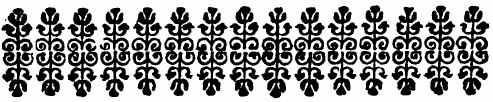
\includegraphics[scale=0.33]{07.erratas.png}
\end{center}
\unskip
\vspace*{-30pt}
{\let\clearpage\relax \chapter{ERRATAS.}}
\chaptermark{}
\sectionmark{}
\lettrine[findent=2pt, nindent=0pt, lines=2]
{P}{A}gina 16. reg. 6. tem Niapykyxoê-\linebreak pemo, lede 
Niapycykixóépemo.\\
Pag. 25. reg. 19. tem agoerabiâra, lede\linebreak ogoerobiâra.\\
Pag. 27. reg. 21. tem ceoroiacegeâbo, lede ceroiacegoâbo.\\
Pag. 49. reg. 8. tem opacatú, lede opacatupe.\\
Pag. 62. reg. 8. tem acepiakine, lede oce-piakine.\\
Pag. 68. reg. 7. tem cetpe catú, lede ceté çupé.\\
Pag. 105. reg. 8. tem oiepiácncá, lede\linebreak oiepiácucá.\\
Pag. 146. reg. 2. tem nhëêugabyagoa-\linebreak
goéra, lede nhëêngabyagoéra.\\
Pag. 155. reg. 14. tem Ipoçang bépe, lede Ipoçangibépe.\\
Pag. 156. reg. 21. tem goemicuagoéra,\linebreak
lede goemicuacugoéra.\\
Pag. 227. reg. 6. tem eremoiecoçúpe, le-\linebreak de
ereimoiecoçúpe.\\
Pag. 247. reg. 6. tem reybâba, lede reymbâba.\\
Pag. 249. reg. ultima. tem onhëâgoâbo, lede enhëãgoâbo.\\
Pag. 315. reg. 21. tem Teomé, lede Teu-\linebreak mé.\\
Pag. 331. reg. 18. \& 333. reg. 7. tem Re-quie\lgS cant, lede 
Requie\lgS cat.
\vspace{\baselineskip}
\begin{center}
    \textit{Além de\lgS tas erratas ha hũas de pouca
    \lgS u\lgS tancia, que por i\lgSS o \lgS enaõ apontaõ.}
\end{center}

\newpage
\vspace*{140pt}
\begin{center}
    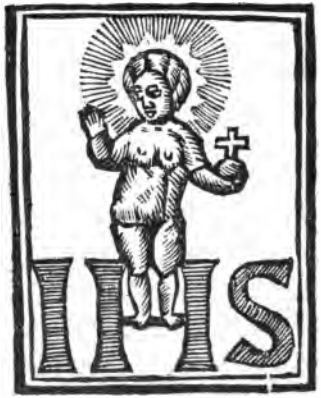
\includegraphics[scale=0.33]{08.jesus.png}
\end{center}
\newpage

\begin{center}
    
\includegraphics[scale=0.36]{09.livro1.png}
    {\large CATECISMO}
    \vspace{5pt}

    {\huge BRASILICO}

    \textit{Da Doutrina Christãa,}
\end{center}
\unskip
\vspace{-30pt}
{\let\clearpage\relax \chapter{\Huge LIVRO I.}}
\unskip
\vspace{-10pt}

\begin{center}
    \textit{Dos primeiros elementos da Fe Chri\lgS tãa,}
\end{center}
\unskip\vspace{-5pt}
\section{Summa dos my\lgS terios, \& \\doutrina Chri\lgS tãa.}

\chaptermark{Summa}
\sectionmark{Da Doutrina Crhi\lgS tãa.}
\unskip\vspace{-5pt}
\par\noindent\rule{\textwidth}{0.4pt}
\unskip\vspace{5pt}
\subsection{Oração do \lgS inal da Cruz.}

%\lettrine[findent =0pt, nindent=0pt, lines=5]
\lettrine[findent =-1pt, nindent=0pt, loversize=-0.1, lraise=0.05, lines=5]
{\zall{S}}{A}NTA Cruz räangâba recé orepy cyrõ iepé, Tupã ore
iár, oré amotarëymbâra çúí. Tû-ba, Täyra, E\lgS pirito Santo
réra pupé. Amen. 
\unskip
\begin{center}
    \unskip
    \textit{Padre No\lgSS o.}
\end{center}
\unskip
\lettrine[findent =4pt, nindent=0pt, lines=2]
{O}{R}é rúb, ybákype tecoár, imöeté pyramo nde réra toicó: Töur
nde Rei-no: Tonhemonhang nderemimotâra yby-pe, ybákype inhemonhânga
iabé: Orérẽ-\linebreak bïú
 âra iabïõ ndoâra eimëeng corí orêbe: Ndenhirõ
oré angaipâba recé orêbe, oré rerecomemoãçâra çupé orénhirõ iabé:
Oremoarucârumé iepé tentaçaõ pupé: Orepy-cyrõ iepé mbäé çüí. Amen.

\subsection{Ave Maria.}
\unskip\vspace*{-12pt}
\lettrine[findent =4pt, nindent=0pt, lines=2]
{A}{V}e Marîa, graça recé tynycémbäé:\linebreak
nde irúnamo iande iâra
recóu: imom-bëú catúpyramo ereicó cunhã çüí; imom-bëú catúpyrabé
ndemembyra JESUS. San-ta Marîa. Tupã cy, etupã monghetá oré 
ïangaipábäe recé cöyr, irã, oré iekyi oré rûmebéno. Amen.

\subsection{Salve Rainha.}

\lettrine[findent =4pt, nindent=0pt, lines=2]
{S}{A}lve Raînha, morauçubâra cy, tecobé, céémbäe, oré
ierobiaçâba, \lgS alve. Ndê-be oroçapucápucai ipëâpyramo Eva 
mem-byramo. Ndébe oronhëangherúr orépöa cémamo, oro iaceguâbo icó
ybytygoâia iaceguâba pupé. Enëĩ ore recé ierureçár\linebreak
ebouĩ nde reçá porauçubâra erobác oré co-ty.
Aë JESUS imombëú catú pyra nde mẽ-byra 
icó iepëaçagoêra cykiré ecepiác ucár, orêbe. Nheranëym,
morauçúb erecoçar\linebreak cëembäé, Virgem Marîa.
Etupã monghetá oré recé,
Santa Marîa Tupã cy, torë angaturâne Chri\lgS to remï-enoĩgoêra
recé oré iecoçubagoâma ri. Amen.

\subsection{Credo.}

\lettrine[findent =2pt, nindent=0pt, lines=2]
{A}{R}obiár Tupã Tûba opácatú mbäe tetiruã monhanga eicatúbä'e,
ybáca, yby abé monhangâra. Arobiár JESUS Chri\lgS to abé Täyra
oiepébäe, acé iâra: E\lgS pirito San-to imonhângâpe pitangamo
onhemonhan-gbäe poêra. Aebäe öár Marîa abábycagoe-rëyma çüí:
Poncio Pilato morobixâbamo cecôreme cerecomémoãbyramo cecóu:\linebreak
ybyrá ioaçâba recé imoiäripyramo cecóu,\linebreak
ijucápyramo, itymimbyramo. Ogoegyb\linebreak
yby apytéripe, âra moçapyra pupé, omanõ-bäe
puêra çüí cecobé iébyri, oieupir ybáky-pe, Tupã Tûba opácatú mbäe
tetiruã monhánga ëicatúbäe, omanõbäe poêra pabẽ\linebreak
recomonhángane. Arobiár E\lgS pirito Santo: Arobiár
Santa Igreja Catholica: Arobiár\linebreak Santos recócatú
ïemoiäó iaöca: Arobiár te-có angaipába recé moroupê Tupã nhirõ:\linebreak
Arobiár acé recobé iebyraõáma: Arobiar\linebreak tecobé opábäeramëyma.
Amen.

\subsection{Artigos da Fé.}

\lettrine[findent =4pt, nindent=0pt, lines=2]
{C}{A}tor\lgS e acéremïerobiarâma.\\ Sete Tupã recé indoâra
nã ëí.

\begin{enumerate}
    \item Arobiar oiepé Tupã opácatú mbäe tetiruã monhânga
    eicatúbäe.
    \item Arobiár túbamo cecó.
    \item Arobiár täyramo cecó.
    \item Arobiár E\lgS irito Santóramo cecó.
    \item Arobiár opacatú mbäe tetiruã monhángáramo cecó.
    \item Arobiár moropycyroánamo cecó.
    \item Arobiár tecobé opábäeramëyma mëéngâramo cecó.
\end{enumerate}
\noindent
Sete JESUS Chri\lgS to ace röó raragoéra rece indoâra nã ëí.
\begin{enumerate}
    \item Arobiár äé Tupã Täyra E\lgS pirito Santo
    i-monhangâpe pitángamo inhemonhangagoéra.
    \item Arobiár Virgem Marîa çüí ïaragoéra, 
    a-babycagoérëymamo cecó pupé memé.
    \item Arobiár acé recé ybyrá ioaçába recé imo-iaripyroéramo,
    ïjucápyroêramo, itymim-byroêramo cecó.
    \item Arobiár yby apytéripe igoegybagoêra, acé rúbypy
    caräíbetá angoéra äépe turâma oçarõbäe renocémagoérabé.
    \item Arobiár âra moçapyra recé cecobé iebyragoéra.
    \item Arobiár ybákype ïieupiragoéra Tupã Tû-ba
    ecatüâba coty cénabé.
    \item Arobiár árapapâne turãgoâma oicobébäe,
    omanõbäepoéra pabẽ recó catúagoéra, cecóangaipgoérabé 
    repymëénga.
\end{enumerate}

\subsection{Mandamentos da Ley de Deos.}

\lettrine[findent =4pt, nindent=0pt, lines=2]
{D}{E}z Tupã acé recómonhangâba.\\
1. Eimöeté oiepé Tupã.
\begin{enumerate}
    \setcounter{enumi}{1}
    \item Anheté erétenhëumé Tupã rêra renõia.
    \item Eimöeté Domingo, âra marã teco abëymabé.
    \item Eimöeté nde rûba, nde cy abé.
    \item Eporapitíümé.
    \item Eporopotarumé.
    \item Emondarõumé
    \item Nde remöémumé abá recé.
    \item Enhemomotárumé nde rapixára remire-có recé.
    \item Enemomotárumé abá mbäe recé.
\end{enumerate}

\noindent Nã ëíbäe pupé pabé aipóbäe rûi.
\begin{enumerate}
    \item Opácatú mbäe tetiruã acé çauçûba çoçé acé Tupã
    rauçûba.
    \item Oieauçûba iábé acé öapixâra rauçûbanó.
\end{enumerate}

\subsection{Mandamentos da Santa Madre Igreja.}

\lettrine[findent =2pt, nindent=0pt, lines=2]
{S}{I}nco Santa Madre Igreja acé recómo-\linebreak nhángâba.
\begin{enumerate}
    \item Domingo recé âra marátecoabëyma recébé Mi\lgSS a 
    rendûba.
    \item Ceixú ïabiõ nhemombëú.
    \item Pa\lgS coa iabiõ Tupã âra.
    \item Santa Madre Igreja iecüacúpoâia 
    iabiõ iecuacûba.
    \item Opácombó iabiõ Tupã çupé oiepé acémbäe moiaóca:
    oemitymbuérypy pupé Tupã potámëéngano.
\end{enumerate}

\subsection{Sacramentos.}
\begin{center}
     \textit{Sete Santa Madre Igreja Sacramentos.}
\end{center}
\comecalista{1.}{2.}{Y}{C}
    {aräîba pupé nhemboiaçûca.\\
    Acé cybápe abaré guaçu nhandy\\\hspace*{14pt} caräíba nonga.}
\begin{enumerate}
    \setcounter{enumi}{2}
    \item Tupã râra.
    \item Nhemombëú.
    \item Acé rëõ ianondé nhandy caräîba râra.
    \item Nhemöabaré.
    \item Mendâra.
\end{enumerate}
\vspace{\baselineskip}

\subsection{Peccados Capitaes.}

\lettrine[findent =2pt, nindent=0pt, lines=2]
{S}{e}te opácatú angaipâba nhemonhángáb ypy.
\begin{enumerate}
    \item Morerobiarëyma.
    \item Tecatëyma.
    \item Moropotâra.
    \item Nhemoyrõ.
    \item Mbäé u, memé cäú eté eté.
    \item Abá mbäé catú möacy.
    \item Tupã recó recé nhemboryryi ëyma.
\end{enumerate}

\subsection{Virtudes contra os \lgS ete peccados.}
\begin{center}
    Sete tecó catu aipó tecó angaipâba robaixoára nã ëí.  
\end{center}
\comecalista{1.}{}{M}{O}
    {rerobiarëyma robaixoâra\\\hspace*{10pt} Nhemöeté ëyma.}
\begin{enumerate}
    \setcounter{enumi}{1}
    \item Tecateyma robaixoára\\\hspace*{40pt} Tecatëyma.
    \item Moropotâra robaixoára\\\hspace*{40pt} Moropotarëyma.
    \item Nhemoyrõ robaixoára\\\hspace*{40pt} Toçânga.
    \item Mbäéu eté, cäú etébé robaixoára\\
    \hspace*{40pt} Oiá nhóte mbäëú, memé cäú.
    \item Abá mbäé catú möacy robaixoára\\\hspace*{40pt}
    Joauçûba.
    \item Tupã recó recé nhemboryryiëyma robaixoâra. Tupã
    recó recé nhemboryryia.
\end{enumerate}

\subsection{Obras de mi\lgS ericordia.}
\begin{center}
    Cator\lgS e acé abá rauçubá çâba.\\
    Sete abá reté recé ndoâra nã ëí.
\end{center}
\comecalista{1.}{2.}{A}{M}
    {byacybôra póia.\\Uceibôra moyú.}
\begin{enumerate}
    \setcounter{enumi}{2}
    \item Icatupendoâra moäôba.
    \item Mbäéacybôra repiâca.
    \item Atâra mombytá.
    \item Imomĩauçubipyra renocêma.
    \item Tëõboêra tyma.
\end{enumerate}

\noindent Sete abá anga recé ndoâra nã ëí.
\begin{enumerate}
    \item Abá çupé recócatúçagoâma mombëú.
    \item Itecócüabëymbäe motecocüâba.
    \item Oicote bẽbae möapycyca.
    \item Oicomemoãbäe renonhêna.
    \item Oguerecomemoãçâra çupé nhirõ.
    \item Abá marã cecó agoérĩ recé nheranëy-\linebreak ma.
    \item Oicobébäe recé omanõbäepoéra recé bé Tupã monghetá.
\end{enumerate}

\subsection{Bemaventuranças.}
\begin{center}
    Oito tecó catu eté rerecoáramo Oporomöĩgobêbäe.    
\end{center}
\unskip
\comecalista{1.}{}{T}{E}
    {có catú eté rerecoâra, öemimotáriboé imbäé ëymbäe,
    imbäéramo ybâca recóune.}
\begin{enumerate}
    \setcounter{enumi}{1}
    \item Tecó catú eté rerecoâra, onheranëymbäe, Aëbäe
    yby oguerecóune.
    \item Tecó catú eté rerecoâra, oiaceõbäe, Aé-bäe
    imöapycykipyramo cecóune.
    \item Tecó catú eté rerecoâra, tecó catú uceitâra
    Aébäe imoytarõbyramo cecóune.
    \item Tecó catú eté rerecoâra, iporaububári-\linebreak bäe,
    Aébäe çauçubâri pyramo cecóune. 
    \item Tecó catú eté rerecoâra, ipyámemoãëy-mbäe,
    Aébäe Tupã ocepiakine.
    \item Tecó catú eté rerecoâra, oporomonhyrõbäe,
    Aébäe Tupã räyri iábamo cecóune.
    \item Tecó catú eté rerecoâra, tecó catú recé
    mbäé poraráçâra, Aébäe ombäéamo ybâ-ca rerecóune.
\end{enumerate}

\subsection{Doẽs do E\lgS pirito Santo.}
\unskip
\vspace*{-2pt}
\begin{center}
    Sete Tupã E\lgS pirito Santo remimëênga.
\end{center}
\unskip
\comecalista{1.}{2.}{T}{U}
    {pã rermimotâra rupí mbäé cüâ-pa. Tecocüâba.}
\begin{enumerate}
    \setcounter{enumi}{2}
    \item Tupã omotecocüâba rupí mbäé mõmbëú.
    \item Myatã.
    \item Mbäécüâba.
    \item Morauçubâra.
    \item Tupã möabá eté.
\end{enumerate}

\subsection{Virtudes Theologaes.}

\begin{center}
    Moçapyr tecó catú Tupã mombegoâba.
\end{center}
\comecalista{1.}{2.}{T}{U}
    {pãrerobiâra.\\Tupã recé ierobiâra}
\begin{enumerate}
    \setcounter{enumi}{2}
    \item Tupã rauçûba
\end{enumerate}

\subsection{Virtudes Cardeaes.}

\begin{center}
    Quatro tecó catú itá.
\end{center}
\comecalista{1.}{2.}{T}{E}
    {có râma ri iepyçacá.\\Abá çupé imbäé mëenga.}
\begin{enumerate}
    \setcounter{enumi}{2}
    \item Myatã.
    \item Mbäé äíba potâra renonhêna.
\end{enumerate}

\subsection{Potenciais da Alma.}

\begin{center}
    Mopyr, mbäé recé acé anga ecatüâba.
\end{center}
\comecalista{1.}{2.}{M}{B}
    {äé recé imäendüaçâba.\\Itecócüâba.}
\vspace{2pt}
\begin{enumerate}
    \setcounter{enumi}{2}
    \item Imbäe potaçâba.
\end{enumerate}

\subsection{Sentidos Corporaes.}
\begin{center}
    Cinco acé mbäé cüapába.
\end{center}
\comecalista{1.}{2.}{M}{A}
    {ẽ\\Mbäé rendúba.}
\vspace{2pt}
\begin{enumerate}
    \setcounter{enumi}{2}
    \item Mbäé retûna.
    \item Mbäé ïupyra räanga.
    \item Mbäé recé mocôca andûba.
\end{enumerate}

\subsection{Novi\lgSS imos.}
\begin{center}
    Quatro abárecó mondycâba.    
\end{center}
\comecalista{1.}{2.}{T}{E}{õ.\\Tupã acé recó cüapâba.}
\begin{enumerate}
    \setcounter{enumi}{2}    
    \item Anhaga ratá.
    \item Ybákype toryba.
\end{enumerate}
\unskip
\vspace{6pt}%\baselineskip}
\subsection{Acto de Contrição.}
\unskip\vspace*{-0.7\baselineskip}
\begin{center}
    Angaipâba möacypâba.
\end{center}
\unskip
\vspace{\baselineskip}
\lettrine[findent =2pt, nindent=0pt, lines=2]
{X}{E}rubiguy Tupã eté, opácatú mbäé çauçubipyra çocé nde
rauçupâpe, icó nde angaturámeté opácatú mbäé iangaturám-bäe
çocé nde recó cüâpa, xe pyápe catú aimö-acy nde nhëenga
abyagoéra, aroirõ opácatû tecó angaipâba, ceroieby potarëyma.
Nde nhirõ tené xêbo, xe iâra JESUS Chri\lgS to ruguy, xe 
anga repymondycâba recé: cecé é guiierobiâbo nde nhirõ recé
taiecoçúb coytene. Amen.

\subsection{Confi\lgSS aõ géral.}

\lettrine[findent =2pt, nindent=0pt, lines=2]
{A}{N}he mombëû Tupã opacatú mbäe tetiruã monhânga ëicatúbäe
çupé, Santa Maria ababycagoerëyma çupébé, S. Miguel Caräíbebé,
Saõ Joaõ Bauti\lgS ta çupebé, Santos Apo\lgS tolos Saõ Pedro,
Saõ Paulo çupébé, opacatpu Santos çupébé, ndêbo bé, Päí aba-ré,
cetanhé xe angaipagoéra recé, tecó angaipába ri xe mäendüáramo,
xe nhëengaíbamo guitecómemoâmo, xe angaipábetéramo. Emonãnamo
aieruré Santa Maria a-babycagoerëyma çupé, Saõ Miguel Caräíbebé,
çupébé, Saõ Joaõ Bauti\lgS ta çupebé, Santos Apo\lgS tolos
Saõ Pedro, Saõ Paulo çupébé, opácatú Santos çupébé, ndêbo bé,
Päí Aba-ré, ipabé xe recé pe tupã Monghtá râma ri.

%Livro 2
\newpage
%\vspace*{150pt}
\begin{center}
    \vspace*{20pt}
    
\includegraphics[scale=0.33]{10.livro2.png}
\end{center}
\unskip
\vspace{-30pt}
{\let\clearpage\relax \chapter{\Huge LIVRO II.}}
\unskip
\vspace{-2pt}
\begin{center}
    {\large CATECISMO}
\end{center}
\unskip
\begin{center}
    Do \lgS inal da Cruz, nome de Chri\lgS taõ,\\
    \& Invocaçaõ dos Santos.\\
    \vspace{6pt}\textit{Com a Explicaçaõ do Padre No\lgSS o,\\
    \& Ave Maria.}
\end{center}
\unskip
\par\noindent\rule{\textwidth}{0.4pt}
\unskip\vspace{-3pt}
\section{DIALOGO I.}
\unskip\vspace{-3pt}
\subsection{Do \lgS inal da Santa Cruz.}

\chaptermark{Dialogo I.}
\sectionmark{do \lgS inal da Cruz.}

%\hspace{-10pt}
\hspace*{-1.5ex}\begin{minipage}[t]{0.16\linewidth}
    Me\lgS tre.\\ \\Di\lgS cip.\\Me\lgS tre.\\ Di\lgS cip.
\end{minipage}
\begin{minipage}[t]{0.95\linewidth}
    \lettrine
    [findent =-2pt, nindent=0pt, loversize=-0.2, lraise=0.05, lines=5]
    {\zall{M}}{B}äépe Chri\lgS taõs iecüa-\linebreak
    \hspace*{2ex}pâba?\\
    Santa Cruz.\\
    Maránamope?\\
    Iárybo omanõmo iandé iâra iandé
    repymëengagoéra recé, anhan-\linebreak
    ga ratá çüí iandé pycyrõ recebé.
\end{minipage}\\

\begin{alternate}
    \item Marã ḯpe acé oiobaçâba?
    \item Santa Cruz räangâba recé orepycyrõ ie-pé,
    Tupã oréiar, oré amotarëymbâra\linebreak
    çüí: Tuba, Täyra, E\lgS pirito Santo rêra\linebreak
    pupé. Amen, ëí.
    \item Maránamopé acé ocybápe iobaçâba möí-ni?
    \item Táxepycyrõ Tupã maenduaçâba äíba çüí oiâbo.
    \item Manránamopé acé oiurúpe çäánghino?
    \item Toipëá Tupã nhëéngmemoã xe iurú çüí oiâbo.
    \item Maránamopé acé opotïápe imöíni?
    \item Táxepëá Tupã tecó angaipâba çüí acé\linebreak
    nhyã çüí ocembäe, oiâbo.
    \item Maránamobé pé acé iobaçâbi?
    \item Santi\lgSS ima Trindade, Tûba, Täyra, E\lgS pirito
    Santo, Moçapyr abá, oiepé Tubã mombeguâbo nhé.
    \item Bäéreme tépé acé iobaçábine?
    \item Mbäé ypyrûnga iabiõ, coêpe marã tecó omöanghecoâime.
    \item Bäéremebépe?
    \item Okér ianondé, opâcagoéripe, ôca çüí o-cémabé.
    \item Oçobacápe acé oemïurâma?
    \item Oçobacáb.
    \item Maránamopé?
    \item Táxemarã ume igoâbo, oiâbo.
    \item Maránamopé acé iobaçáb etá etáone?
    \item Táxepycyrõ Tupã xe çumarã çüí coépe marã xerecoápe, oiâbo.
    \item Abá pe acé çumarã?
    \item Anhânga.
    \item oierokype acé Cruz çupé?
    \item Oieroky.
    \item Marã, ybyrá çupé nhépe, acé ierokyu?
    \item Näani, çaangabijára çupéé, cecé omäen-düáramo.
    \item Abápe Cruz räangâbiâra?
    \item Iandé iâra JESUS Chri\lgS to.
    \item Maránamo pé?
    \item Cecé imboiaripyramo omanômo oie-\linebreak 
    möatã agoéra recé.
    \item Oierokype acé iandé iâra räangâba çu-pé, Santa Maria
    Tupã cy räangâba çupé, Santos ybakypendoára räangâba çupébé?
    \item Oieroky.
    \item Ybákype oicóbäe möeté iabé pe acé çä-angâba möetéo?
    \item Iiabé.
    \item Marã, itánhépe coipó ybyrá, nhäûma çüí imonhanghimbyra
    nhé pe acé oimoeté?
    \item Näâni, çäangabijâra é: çäangábamo cecó reme, cecé
    omäendüáramo.
\end{alternate}

\par\noindent\rule{\textwidth}{0.4pt}
\unskip\vspace{5pt}
\section{DIALOGO II.}
\unskip\vspace{-3pt}
\subsection{Do Nome de Chri\lgS taõ.}

\chaptermark{Dialogo II.}
\sectionmark{do Nome de Chri\lgS taõ.}

\comecalista{M.}{}{M}{A}{rápe imongaräíbipyra renõidábeté?}
\vspace{4pt}
\begin{altereven}
    \item Chri\lgS taõs.
    \item Maránamopé?
    \item Chri\lgS to iande iâra rerobiaçáramo cecóreme, cecó
    mombeguáramo cecóreme.
    \item Niapycykixóépemo cerobiaçâra opyápe nhóte cerobiâbo?
    \item Niapycykixóemo, omanõmo tiruá cerobiámo.
    \item Iandé iâra JESUS Chri\lgS to çüí.
    \item Abápe JESUS Chri\lgS to?
    \item Tupã eté, apŷabeté iandé iabêbé.
    \item Manránamopé acé Tupã eté, ïeú ixupé?
    \item Tupã Tûba räyreté oiepêbäêramo cecóreme.
    \item Aêpe marã apyábetêramo cecóu iandê-iabê?
    \item Cunhã angaturâma ababycagoerëyma\linebreak
    Santa Maria Ceríbäe membyramo cecó\linebreak reme.
    \item Nixyítepe Tupã etéramo oicôbo?
    \item Nixui, nacetéi, nïypyi Tupã etéramo oi-côbo.
    \item Natûbi tépé apyábetéramo oicôbo?
    \item Na tûbi, onhemonhanghé ocy iatoĩby-rëyma righépe.
\end{altereven}

\vspace{3pt}
\par\noindent\rule{\textwidth}{0.4pt}
\unskip\vspace{5pt}
\section{DIALOGO III.}
\unskip\vspace{-3pt}
\subsection{Do \lgS anti\lgSS imo Nome de Je\lgS us, \&
            invocaçaõ dos Santos.}

\chaptermark{Dialogo III.}
\sectionmark{da invocaçaõ dos Santos.}

\comecalista{M.}{D.}{A}{B}
    {ápe acé ocenoĩ oicótebêmo?\\
    JESUS ocenoĩ.}
\begin{alternate}
    \item Maránamopé?
    \item Táxe pycyrõ marã tecó çüí, oiábo.
    \item Marã oiâbo pé acé JESUS ïeú?
    \item Moropycyrõâna oiâbo.
    \item Oierokype acé JESUS éreme?
    \item Oierokype.
    \item Marã éreme bépé acé ierokyo?
    \item Santa Maria éreme.
    \item Maránamopé?
    \item Tupã cyramo cecóreme nhé.
    \item Abá çupéé acé ierúréo öeté maranëyma-õâma recé,
    öanga recocaturâma recébé?
    \item Tupẽ çupé.
\end{alternate}
\begin{alternate}[parsep=-5.4pt]
    \item Abápe acé recé Tupã manghetaçáramo cecóu?
    \item Santa Maria Tupã cy, Caräíbebé aceraroâna abé.
    \item Acerarõánamo tepé Caräíbebé recóu?
    \item Acerarõánamo.
    \item Oiabiõpé acé cerecóu?
    \item Oiabiõ.
    \item Mbäérâma recépe Tupã imëenghi acébé?
    \item Acé çumarã çüí acé rarõ agoâma recé.
    \item Mbäé, mbäé çüípe acerarõu?
    \item Anhánga çüí, tecó angaipâba çüí, mbäé äíba çüí bé.
    \item Marã ëípe acé caräíbebé öaroâna mon-ghetâbo?
    \item Caräíbebé xe rarõâna, xe pëá iepé mbäé äíba çüí
    cori, Tupã remimotâra rupí xe\linebreak moĩgôbo, ëí.
    \item Abá, abápe acé recé Tupã monghetaçáramo cecóu?
    \item Santos etá ybákype tecoâra.
    \item Emonánamo pé acé ieruréo Santos etá çupé.
    \item Emonánamo, memé ogueriiâra çupé.
    \item Marã ëípe acé ixupe oierurêbo?
    \item Peimonghetá Tupã iandé iâra ixêbo, taxerauçubár ëí.
\end{alternate}
\begin{alternate}[leftmargin=8pt]
    \item Mbäé mbäéremepé acé ieruréo ixupé?
    \item Iepínhé, memé ïâra áreme no.
    \item Maránamope acé Sãtos âra cüabi, imöetêbo, ipupé
    toryba monhânga?
    \item Ybákype Tupã imöeté catú recé omäen-düáramo.
    \item Maránamo bépé?
    \item Cecó catúgoêra rupi oicó potá taicó catúïiabébé
    cá oiâbo.
    \item Maránamobépé?
    \item Çauçûpa, totupãmonghetá xe recé ixe
    oguauçûme,oiâbo,ixe omöetéreme oiâbo.
    \item Mbäerama rí bépe acé Santos âra cüâbi?
    \item Tupã ixupé tecó catú mëengâra möeté agoâma recé.
    \item Marãngatúpe acé recóu Tupã ókype oikeâbo?
    \item Oieypyi y caräíba pupé.
    \item Mbäé râma recépé?
    \item Anhânga monhegoacemãõâma recé.
    \item Mbäé râma recébépe?
    \item Acé angaipá mirĩ recé, acêbo Tupã nhi-rõ aõgoâma recé.
    \item Marãgatúpe acé recóu ipipé oieypyia?
    \item Oimöacy catú öangaipâba opyápe.
    \item Marã ëípe acé Tupã okype oikeâbo, y caräíba pupé 
    oieyoyîa? 
    \item Y imongaräíbipyra toicó xe anga 
    recobéçáramo, tomonhegoacémucár anhân-ga xe çüí. Amen 
    Je\lgS us, ëí.
    \item Ocypyibépe acé tyby y caräíba pupé?
    \item Ocypyi bé.
    \item Mbäérâma recépe?
    \item Tonhegoacém anhânga ixüí, oiâbo.
    \item Marã ëípe acé oké ianondé, Tupã mon-ghetâbo.
    \item Xe iár JESUS Chri\lgS to, nde réra pupé a-nhenõg
    guiképotá, äé taxerobaçáb, äé taxerarõ, äé abé taxepycyrõ,
    äe abé taxereraçó ogorypápe, ëí.
    \item Marã ëípe acé opâca roire?
    \item Xe iár JESUS Chri\lgS to eceçapé corí xe\linebreak
    anga reçá, taiabyuméné icó âra pupé nde nhëênga,
    nde remimotâra rupí catú xe\linebreak moingó iepé corí, ëí.
\end{alternate}

\vspace{2pt}
\par\noindent\rule{\textwidth}{0.4pt}
\unskip\vspace*{-4pt}
\section{DIALOGO IV.}
\unskip\vspace{-3pt}
\subsection{Do Padre No\lgSS o.}

\chaptermark{Dialogo IV.}
\sectionmark{Do Padre No\lgSS o.}
\vspace*{-6pt}
\comecalista{M.}{D.}{M}{A}
    {rã ëípe acé Tupã monghetâbo?\\
    Oré rúb, ybákype tecoár, ëí.}
\begin{alternate}
    \item Abápe aipóbäé oimonháng erímbäé 
    çä-anghypyâbo?
    \item Iandé iâra JESUS Chri\lgS to äé oçäang\linebreak
    erímbäé oiurú rupí catú.
    \item Mbäérâma recépe?
    \item Tupã monghetá recé iandé mböébo nhé.
    \item Onhemoçainân pabẽpe Chri\lgS taõs aipó-bäé
    cüabaõáma recé?
    \item Ouhemoçainân pabẽ.
    \item Tupã çupéé acé orerúb ïéu?
    \item Tupã çupé.
    \item Marãpe acé rubamo cecóu?
    \item Acé monhangaretéramo oicôbo.
    \item Marãpe acé monhânghi?
    \item Nã mbäé rüã oimonháng acé angamo,
    onhëênga pupé é imonhânghi.
    \item Nace rûba rüã tepé acé reté oimonháng?
    \item Acé rûba oimonháng bïã, Tupã imo-\linebreak
    nhânga potaçâpe é.
    \item Marã oicôbo bépe Tupã acé rúbamo cecóu?
    \item Acé rûba, acé cy, acé rauçûba çocé, acé rauçûpa,
    öäyretêramo acé rerecôbo.
    \item Marã ëípe acé opyápe Tupã çupé, orerúb, oiâbo?
    \item Taimöeté catú xe rûba cá, taçauçub ca-tú,
    taçapiar catú cá, oiâbo.
    \item Otĩ nhémo cerã iangaipábäé, oré rúb,\linebreak oiâbo
    Tupã çupé?
    \item Otĩ nhémó anhé, otecocüábamo emó.
    \item Marãnamo pe?
    \item Naçapiár icó xerúbeté, oiâbo, naiár icó
    cecó angaturâma, oiâbo.
    \item Marã ëíbépé acé opyápe, oré rúb, oiâbo Tupã çupé.
    \item Arobiár catú ce rûba Tupã recé, ëí: äé xererecó,
    äé xepycyrõ, äé xerecotebẽçâba oimëéng ixêbonê, ëí.
    \item Oierobiácatúpe acé Tupã recé aipó oiâ-bo?
    \item Oierobiácatú, abábiã é öäyra oguerecó catú,
    memétipó Tupã mbäé tetiruã iára-mo oicóbäé acé rauçubáne,
    oiâbo.
    \item Marãnamo pé acé orérúb ïeú, Xerûb öénhóteëyma?
    \item Oioanametéramo pabẽ, Tupã räyretéra-mo pabẽ cecó
    cüâpa, oiöauçûba potá.
\end{alternate}

\subsection{Que e\lgS tàs nos Ceos.}
\unskip\vspace*{-0.7\baselineskip}
\comecalista{M.}{D.}{M}{A}
    {mópe Tupã recóu?\\
    Ybákype, ybype, opacatú mbäé\linebreak mopôri.}
\begin{alternate}
    \item Maránamo tépé, ybákype tecóar, acé ïeú ixupe?
    \item Ybakype é iangaturambäé çupé iepiacu-cá potéreme.
    \item Maránamobépé.
    \item Ybákype é ogubeté, öemimotáreté recó-cüâpa, acé
    Tupã repiacäûbi, yby árybo\linebreak ocoábäé reroyrómo.
    \item Marã ëípe acé opyápe ybâca recé omäêmoné?
    \item Ybákype é Tupã xe rubeté recóu mã ëí-né, açó
    temo xe rûba pyri, xe retametépe mã, ëíné.
    \item Naceretâma rüãtepé icó yby acé recoâ-ba?
    \item Näani, ybâca porâma recé é Tupã acé\linebreak
    monhânghi: atáramo é acé recóu icó yby pupé.
\end{alternate}
\unskip\vspace*{-0.7\baselineskip}
\subsection{Santificado \lgS eja o teu Nome.}
\unskip\vspace*{-0.7\baselineskip}
\comecalista{M.}{}{M}{B}
    {oby mbäé recé pe acé ierureó,\\
    \hspace*{10pt}orérúb ëíbäé räânga?}
\begin{altereven}
    \item Sete mbaé recé.
    \item Marã ëípe ïypy?
    \item Imöeté pyramo nde rêra toicó, ëí.
    \item Marã oiâbo  pé acé aipó ïéu Tupã çupé?
    \item Tandererobiá pabẽ abá, ogúbamo, omo-nhangáramo
    nde recó cüâpa, nde möetê-bo, oiâbo.
    \item Abá abápe Tupã réra oimöeté ucár?
    \item Chri\lgS taõs inhëênga rupí tecoâra.
    \item Marã iabépe?
    \item Chri\lgS taõs recó catú repiâca é ipó, 
    imongarâibipyrëyma Tupã mombëú catú, ce-có recé 
    onhe momotá.
    \item Aëpe Chri\lgS taõs Tupã nhëêngabyâra,\linebreak
    marã? 
    \item Aë ipó Tupã noimöangaturâmi imonga-räíbipyrëyma
    çupé, cecó potárucáreyma.
\end{altereven}

\subsection{Venha a nós o teu Reino.}

\comecalista{M.}{D.}{M}{A}
    {rã ëípe amó äé acé ierureçâba?\\
    Tour nde Reino, ëí.}
\begin{alternate}
    \item Marã oiâbo pé acé aipó ïeú?
    \item Nde nhõ tore recó iepé, oré rubixácatúramo
    eicôbo, oiâbo.
    \item Marã oecó potápe acé aipó ïéu?
    \item Tupã boiáramo nhõ oicópotá, inhëên-ga rapiá potá,
    anhânga oiáramo cecó potarëyma.
    \item Marã oicôbo tepé acé anhânga rembï-\linebreak auçúbamo
    cecóu?
    \item Öangaipábamo, Tupã nhëênga abyâbo.
    \item Marã oiâbo bépe acé, Töúr nde Reino, ïéu?
    \item Toroguacém te ybákype nde recóabetê-pe, nde
    iepuacucáçápe, oiâbo.
    \item Mbäé pe Tupã oimëéng acêbe ybákype ne?
    \item Tecobé opabäéramëyma.
    \item Erimbäé pe né?
    \item Acé rëõ riré ybákype acé ânga reraçôbo.
    \item Aëpe acé reté rëombuêra marã?
    \item Arapábiré imöingobéiebyri opyri cera-\linebreak çôbo
    auieramanhé ne
\end{alternate}

\subsection{Seja feita a tua vontade, \&c.}

\comecalista{M.}{D.}{M}{A}
    {rã ëípe amó äé.\\
    Tonhemonhang nde remomotâra ybype
    ybákype inhemonhang iabé, ëí.}
\begin{alternate}
    \item Marã oiâbope acé aipó ïéu?
    \item Toicó pabẽ ybypeçoâra nde remimotâra
    rupí ybakygoâra recó iabé oiâbo.
    \item Noimomarã mirĩ angâipe ybakygoâra\linebreak
    Tupã remimotára?
    \item Näanagai: acé iangaipábäé ipó icó yby pé Tupã
    remimotâra noimonhânghi.
    \item Marãngatúpé Tupẽ acé recó oipotar?
    \item Oipotár acé agoerabiâra, öauçûba, öecö-abyëyma.
    \item Marãnamobépe acé tonhemonháng nde remimotára,
    ïéu Tupã çupé?
    \item Mbäé poxy ogoeté remimotâra rupi oicópotarëyma;
    anhânga remimotâra morãbué potábé no.
    \item Mbäé mbäépe anhânga oipotár?
    \item Acé Tupã nhëênga aby, öatápe acé rera-çó potá;
    ybákype Tupã rorypápe iandé çó potarëyma.
\end{alternate}

\subsection{O paõ no\lgSS o de cada dia, \&c.}

\comecalista{M.}{D.}{M}{A}
    {rã ëípe amó äé acé ieruréçâba?\\
    Oré rembïú âra iabiõdoâra eimë-éng cori orebê, ëí.}
\begin{alternate}
    \item Mbäé pïã rembïú acé ierureçâba?
    \item Acé reté remïurâma, acé ânga remïrâma abé.
    \item Mbäé pé acé reté rembïú?
    \item Mbäé ïupyra acé recobé çãogoâma recé Tupã
    remimonhangoêra.
    \item Nacé rüãpe oemïurâma oimonhâng?
    \item Näâni, acé té onhemoçainán nhóte; Tu-pã äé oimonhâng
    acé moiecoçúbucá.
    \item Mbäé mbäé pé acé ânga rembïú?
    \item Tupã goty acé ioauçûba, acé ânga recobêçâba.
    \item Mbäé abêpé?
    \item Iandé iâra JESUS Chri\lgS to reté.
    \item Marã iabétepé acé ânga ïúi?
    \item Acêbe abaré Snti\lgSS imo Sacramento më-engheme,
    acé Tupã ráreme.
    \item Oiucêi catú cerã Tupã rauçupâra ânga Santi\lgSS imo
    Sacramento; corí corí äú iguâ-bo ïepí?
    \item Oiucéi catú, ïiucêia rerecôbo é ipó Tupã nhëengabyeyme.
    \item Mbäé abêpe acé ânga rembïú?
    \item Tupã nhëénga acé mböeçâba.
    \item Maránamopé acé mïú ïeú ixupé?
    \item Cecé acé ânga recobêreme.
\end{alternate}
\unskip\vspace*{-0.7\baselineskip}
\subsection{Perdoanos no\lgSS as dividas, \&c.}
\unskip\vspace*{-0.7\baselineskip}
\comecalista{M.}{D.}{M}{A}
{rã ëípe amó äé?\\ Nde nhyrõ oré angaipâba recé
orébe, ore rececó memoãçâra çupé oré nhyrõ iabé, ëí.}
\begin{alternate}
    \item Onhemoyrõ tepé Tupã acêbe amómé?
    \item Onhemoyrõ, acé anganpâme, acé rauçú pëâbo.
    \item Marãpe acé recóu imonhyrômo?
    \item Onhemomborëauçub öangaipâba möa-cyâbo,
    ceroiacegeâbo, ceroieby potarëy-\linebreak ma.
    \item Marã ëípe acé opyápe imöacyâbo?
    \item Xe angaipábeté, Tupã xerubeté nhëengabyâbo,
    imöetêëyma mã, ëí, çauçubëyma ceçá pe
    nhé xe poxyramo mã, ëí.
    \item Noimöepyixôépe acé öangaipagoêra imöacy
    apyrixoáramo ne?
    \item Oimöepy, oiecüacûpa, onhenupã nupâ-mo, Tupã recé
    mbäé mëênga. Tupã recé mbäé parorâbo, Tupã recé abá
    rauçubá.
    \item Aëpe icó âra pupé cepy cykëyme?
    \item Purgatorio pé é acé çou cepy mondycá-ne?
    \item Marã ëípé acé Tupã mombúpotá?
    \item Oré rerecomemoãçâra çupé oré nhirõ\linebreak iabé,
    nde nhirõ orêbe, ëí.
    \item Oipotá catú cerá Turã iandé rerecó memoãçára
    çupé iandé nhirõ?
    \item Oipotá catú, emonã acêrecó recé, acé rauçucatuâbo,
    acébo oierecoácatúramo. 
    \item Marã oecó pupépe erímbäé aipó recé iandé mböeú?
    \item Iandé onhëênga abyâra recé oieiucäucá.
    \item Marã oicôbo bépe?
    \item Santa Cruz omoiaçápe oiucaçâra recé\linebreak
    oierurêbo, nde nhirõ ixupé oiâbo ogûba Tupã çupé.
\end{alternate}
\unskip\vspace*{-0.7\baselineskip}
\subsection{Naõ nos deixes cair em tentaçaõ.}
\unskip\vspace*{-0.7\baselineskip}
\comecalista{M.}{D.}{M}{A}
{rã ëípe amó äé?\\ Oré moarucarumé iepé tentaçaõ pupé, ëí.}
\begin{alternate}
    \item Mbäé çupêpe acé tentaçaõ ïeú?
    \item Anhânga ace räânga çupé, acé röó acé\linebreak momoxy
    potâra çupêbé.
    \item Mbäé çupébé pe?
    \item Mbäé acy çupé, abá acé rerecómemoã çu-pé, mbäé
    tetiruã oemimborarátyba çupé.
    \item Oipotáripe Tupã aipobäé acpe iporarâ?
    \item Oipotár.
    \item Mabäérâma rípe?
    \item Toimöepy öangaipâba yby pupé, oiâbo, ybákype
    acé reraçó çapyá potá.
    \item Marã oiâbo bépe acé aipó ïeú?
    \item Oré mopyatãgatú iepé, toröâruméné nde nhëenga
    abyâbo, oiâbo.
    \item Acé äé cerã öápotâri Tupã nhëênga aby tentaçaõ
    iâba pupé?
    \item Acé äé.
    \item Marã oicôbo pé?
    \item Mbäé oemimborarátyba çupé ogoçan-\linebreak ghëymamo.
    \item Nã anhânga rüã tepé acé mböar tecó angaipâba pupé? 
    \item Nã anhânga rüã: acé räáng räáng nhóte anhânga;
    acé äé onhemöabangá imbory-pa, opyatã potareymamo.
    \item Nhũçâna abyarëyma nhé cerã tentaçaõ,
    anhánga, acé röó abé acé räánga?
    \item Nhũçâna abyarëyma nhé.
    \item Marã iabépé?
    \item Emäẽ tacó, nhũçâna öin nhóte: guyrá äé
\end{alternate}
\hspace*{5pt}oçó ipupé öâbo: ã çöó iabé ipó acê oemi-
\hspace*{5pt}motâra rupí é
    iâri angaipâba pupé.
\begin{alternate}
    \item Ndeitëé nipó acé Tupã çupé, xe pytybõ
    iepé oiâbo iepí?
    \item Ndeitëé: Tupã opytybõneme é acé pyatã gatúramo, 
    öânga çumarã reityca.        
\end{alternate}

\subsection{Mas livranos do mal. Amen.}

\comecalista{M.}{D.}{M}{A}
{rã ëípe amó äé?\\ Oré pycyrõ iepé mbäé äíba çüí, ëí.}
\begin{alternate}
    \item Mbäé çupébé acé mbäé äíba ïeú?
    \item Anhânga acé ânga çumurã acé räânga\linebreak çupé.
    \item Mbäé çupébépe?
    \item Peccado, Tupã nhëênga aby çupé.
    \item Mbäé äíbeté catú cerã peccado?
    \item Mbäé äíbeté catú: cecé é Päí Tupã acé rauçú pëáo,
    anhânga pópe acé mëênga.
    \item Ndeitëé nipó acé peccado Tupã nhëên-ga aby möabäetêbo
    tëõ çocé, mbäé teti-ruã çocé?
    \item Ndeitëé.
    \item Mbäé çupé bépe acé mbäé äîba ïeú?
    \item Anhânga ratá çupé, bóia, iagoâra, mbäé acy,
    mbaräára çupé, opábenhé acé ânga çumarã, coipó acé reté
    rupiâra çupé. Amẽ.
    \item Marã oiâbo pe acé Amen ïeú?
    \item Tipór aipó xe ierureçâba oiâbo.
    \item Maranámope acé çäânghi Tupã mõghetâbo?
    \item Tupã ace ierureçâba mopôra potá.
    \item Marãgatúpe ace recóu Tupã ogoapiarãogoâma recé ne?
    \item Oierobiá catú cecé, oieruré pöírëymane.
    \item Mbäépe acé ocenoĩ ixupé oierobiaçába-mo.
    \item Iandé iâra JESUS Chri\lgS to rëõ agoéra, ce-cé
    ipó Tupã xerauçubárine rëá, oiâbo. 
\end{alternate}

\vspace{6pt}
\par\noindent\rule{\textwidth}{0.4pt}
\unskip\vspace*{6pt}
\section{DIALOGO V.}
%\unskip\vspace{-3pt}
\subsection{Da Ave Maria.}

\chaptermark{Dialogo V.}
\sectionmark{Do Padre No\lgSS o.}
\vspace*{2pt}
\comecalista{M.}{}{M}{A}
    {rã ëípe acé Santa Maria monghetâbo?}
\begin{altereven}
    \item Ave María, ëí.
    \item Marã ,näé cunhãpe Santa María?
    \item Cunhã angaturámeté ababycagoerëyma Tupã Täyra cy,
    ybákype oicóbäe.
    \item Abápe aipó Ave María oçaánghypy erímbäé?
    \item Caräíbebé.
    \item Erímbäépe çäanghi?
    \item Santa María çupé Tupã nhëénga rerú,\linebreak
    Ave, eicobé catú oiâbo ixupé? 
    \item Mbäé Tupã nhëênga oguerúr ixupé?
    \item Ereicó xecyramo ne, Tupã Täyra é, 
    oguerúr erímbäé.
    \item Marã oicôbope Tupã Täyra ocyramo \linebreak
    Santa María râri?
    \item Cyghépe pitángamo onhemonhânga.
    \item Marã Santa María recóreme pé caräí-\linebreak
    bébé reikêu ixupé?
    \item Tupã monghetá cêneme.
    \item Ocepiác pé Santa María äé caräíbebe,\linebreak
    monghetáreme?
    \item Ocepiác.
    \item Marãpe cepiaki cetëëymbäéramo cecó-\linebreak
    reme?
    \item Acé iabé catú nhé caräíbebé iepiacurâri ixupé,
    cunumĩ guaçú porangatú iabé nhé.
    \item Oieroky catúpe Santa Maria çupé imon-ghetâbo?
    \item Oieroky catú, Tupã cyramo cecôrâma\linebreak
    cüâpa, imöeté catuâbo. 
    \item Memêtipó acé ixupé oierokyâbone?
    \item Memé, ogoendypyâëybo catú acé rêni\linebreak
    imonghetâbo ne.
\end{altereven}
\sectionmark{Da Ave Maria.}
\newpage

\subsection{Chea de Graça.}
\vspace*{2pt}
\comecalista{M.}{D.}{M}{A}
    {rã ëíbêpe Caräíbebé ixupé?
     Graça recé tynycêmbäe, ëí.}
\begin{alternate}
    \item Mbäé çupépé acé graça ïéu?
    \item Mbäé catú eté amó acé ânga çupé Tupã
    remimëênga öecó potaçâba rupí acé möingoçâba çupé.
    \item Marã iabépe acé recóu Graça rerecôbo?
    \item Tupã remiauçucatúramo cecóu, Tupã\linebreak öauçûba
    pöepyca, çauçûpanó.
    \item Marã iabébépé?
    \item Ipyatã mbäé äíba çocé Tupã nhëênga\linebreak abypëabo,
    Tupã recé marã tecó pouçibëy-ma.
    \item Ybákype oçobäérâma nhõpe graça oguerecó?
    \item Ybákype oçobäérâma nhõ.
    \item Doieiyipe amóneme acé ânga çüí?
    \item Oieiyi, angaipâba acé imonhángheme.
    \item Marãteimpe acé ânga imocanhêmi ré?
    \item Ipoxy, imembéc, anhânga poguyribo nhé
    cecóu, çatápe oçó ianondé.
    \item Tynycêgatípé Santa Maria aipó mbäé eté Graça iâba recé?
    \item Tynycêngatu: äé racó noiabymirĩ angái Tupã nhëênga
    erímbäé.
    \item Marã ëípe acé opyápe aipó oiâbo ixupé?
    \item Xerauçubucá iepé Tupã çupé ëí, togoenocém mbäé
    äíba xe ânga çüí, oporöau-çûba recé imoynycêma, ëí. 
\end{alternate}

\subsection{O Senhor eh contigo.}
\vspace*{-2pt}
\comecalista{M.}{}{M}{A}
    {rã ëíbêpe Caräíbebê Santa Ma-ría çupé?}
\begin{altereven}
    \item Nde irúnamo iandé iâra recôu, ëí.
    \item Marãgatú etépe Tupã recõu Santa Ma-ría irúnamo?
    \item Iânga pupé, inhyâme, ipyápe.
    \item Marãiabépe?
    \item Memé nhé TUpã recé omäendüáramo, çauçûpa, ixupe
    onhëênga, ceçápe xe recóu rëĩ, oiâbo.
    \item Deitëé ipó tecó catú öirëymeté catuâbo iânga çüí?
    \item Deitëé ipó.
    \item Marã abépe Tupã recóu Sãta María irúnamo?
    \item Cyghépe iandé röó raçâpe.
\end{altereven}
\subsection{Benta es tu, \&c.}
\vspace*{-2pt}
\comecalista{M.}{D.}{M}{A}
    {rã ëíbêpe Caräíbebé ixupé?
    Imombëú catupyramo ereicó cunhã çüí, ëí.}
\begin{alternate}
    \item Iangaturãgatú eté cerã Santa Maria opacatú cunhã çüí?
    \item Iangaturãgatú eté, tecó catú oioupé Tu-pã
    remëengoéra mocanhemëyma.
    \item Marã oicôbo bépe iangaturánamo?
    \item Iandé rubypy recó angaipagoéra acé\linebreak
    nhemonhânga pabẽ pupé onhemonhan-ghëyma.
    \item Marã oicôbo bépe?
    \item Ababycabëymamo öecó pupênhé, Tupã cyramo 
    oicôbo, imböá tirüã, imboár ëymebé, äéramëĩ imböá riré
    omaranëyma-mo.
    \item Ara recó pucúipe abá imombëú catúne?
    \item Ara recó pucui.
\end{alternate}
\unskip\vspace*{-10pt}
\subsection{Bento he o fruto, \&c.}
\unskip\vspace*{-12pt}
\comecalista{M.}{}{M}{A}
    {rã ëíbépe acé Santa María mõ-\\
    ghetâbo?}
\begin{altereven}
    \item Imembëú catúpyra abé nde membyra JESUS, ëí.
    \item Abá nhëengoêra pe aipó?
    \item Santa I\lgS abel ianâma nhëengoêra.
    \item Erímbäé pé çäanghi?
    \item Oçûba Santa María çóreme.
    \item Erímbäepe îxóu ixûba?
    \item Imembyra Saõ Joaõ rurúreme.
    \item Oïn üãpé Tupã Santa Maria ryghépe,\linebreak
    \newpage iandé röó raçâpe Santa I\lgS abel pyri ixóre-me?
    \item oïn üã.
    \item Marã oicôbopé acé Santa María çupé\linebreak
    iieauçubucâri?
    \item Imembyra JESUS mombëú catûabo.
    \item Marãgatú etêpe acé imombëú catuú?
    \item Tupã etêramo cecó mombegoâbo, mbäé tetiruã 
    monhangáramo, iandé iâramo ce-có mombegoâbo.
    \item Marãiabêpebé?
    \item Cunumínamo inhemonhangagoêra, ïâragoêra, cëõ
    agoêra cecobe iebyagoêra,\linebreak opacatú cecó angaturâma
    monbegoâbo, abá çupé cerobiárucá.
\end{altereven}
\subsection{Santa Maria, \&c.}
\unskip\vspace*{2pt}
\comecalista{M.}{}{M}{A}
    {rã ëí bépe acé Santa María mõ-\\
    ghetápapâpe?}
\begin{altereven}
    \item Santa Maria Tupã cy, etupãmonghetá\linebreak
    oré angaipâbäé recé, coyr, irã, oré iekyi\linebreak
    oré rûme bénó, ëí.
    \item Çory catúpe Santa Maria, Tupã cy oio-upe éreme?
    \item Çory catú, Tupã cyramo oicôbo é iangaturambábetéramo
    cecóu.
    \item Marã pé acé rerecóu Tupã cyramo oecó rece omäendüáramo?
    \item Omembyra Tupã acé angaipâba recé\linebreak acêbe 
    inhemoyrõb6aé oimonhyrõ, anhân-ga ratâpe acé mondóucarëyma.
    \item Marã abépe acé rerecóu?
    \item Oioupé acé ieruréreme acé rauçubâri,\linebreak
    acé porëauçubóki, tecó poxy pupé acé\linebreak möarucárëymi.
    \item Mbäéreme pé emonã cecóu?
    \item Cöyr, icó âra pupé acé recó pûkui, memé
    ipó acé iekyi acé rûme.
    \item Aëreme  ipó acé pytybõ gatú ybákype\linebreak
    acé reraçó potá?
    \item Aëreme é acé çüí oiëiyeyma, anhânga\linebreak
    mondyia, ixüí acé ânga pycyrômo.
    \item Acé cyramobé cerã Tupã ocy möingóu?
    \item Acé cyramo bé, emonánamo é xe cy acé ëí ixupé.
    \item Maránamo pé.
    \item Acé cy omembypitânga rauçûba çoçé acé rauçûme nhé. 
    \item Mbäépé Santa Maria acé rauçupâba?
    \item Imembyra iandé iâra JESUS Chri\lgS to rëõgoêra.
    \item Marãiabépe?
    \item Cecobérâma mëêng potá erímbäé xe\linebreak \newpage
    membyra tëõ poraráo rëĩ, ëí nhe acêbe\linebreak
    omembyramo acé rerecôbo.
    \item Oierobiá catúpe acé Santa Marîa recé xe cy oiâbo ixupé?
    \item Oierobiá catú, náxe reroyroy xoé corí xe cyne,
    oiâbo, naxerauçú pöíri xoéne, oiâ-bo.
    \item Marã gatúpe acé recóu cecó pöepyca?
    \item Oçauçú catú opyápe, ocepiacäúb, oçapiá catú imenbyra
    JESUS nhëênga.
    \item Oipotá catúpe Santa Marîa acé omembyra JESUS nhëênga
    rapiâra?
    \item  Oipotá catú emonã acé recó, äé ipó ïapy-cycábetêramo
    cecóu.
    \item Marã ëípe acé opyápe, etupãmonghetá oré iangaipâbäé
    recé, oiâbo ixupé?
    \item Ore angaipáb oré, ëí, oromöabáeté nde membyra oré
    angaipâbamo, ëí, eiorí ïa-\linebreak áeté ôca imonhyrômo, ëí.
    \item Oimonghetá pyypyyípe acé Santa Ma-rîa, ixupé
    oierurêboné?
    \item Oimonghetá pyypyyi, Ave Marîa räânga iepíné.
    \item Maránamo pé?
    \item Tecótebẽbóramo oicôbo, taxe moiecoçúb, oiâbo.
    \item Maránamo bépe?
    \item Oänga curumã omboéäíme, taxéporauçuberecó, taxé rarõ
    memé iepí, oiâbo.
    \item Iäpycyki catú cerã acé imonghetâbo?
    \item Iäpycyki catú, çauçúba rerecôbo, cecó\linebreak
    catú rupí oicópotá, ocy angaturâma remimotâra abypotarëyma.
\end{altereven}

\begin{center}
    \vspace*{20pt}
    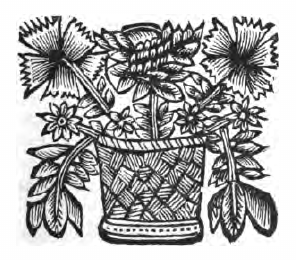
\includegraphics[scale=0.66]{11.livro2_fim.png}
\end{center}
\newpage

%\vspace*{150pt}
\begin{center}
    \vspace*{20pt}
    
\includegraphics[scale=0.33]{12.livro3.png}
\end{center}
\unskip
\vspace{-30pt}
{\let\clearpage\relax \chapter{\Huge LIVRO III.}}
\unskip
\vspace{-2pt}
\begin{center}
    {\large CATECISMO}
\end{center}
\unskip
\begin{center}
    Do\lgS mi\lgS terios que \lgS e contém\\
    no Credo.
\end{center}
\unskip
\par\noindent\rule{\textwidth}{0.4pt}
\unskip\vspace{-3pt}
\section{DIALOGO I.}
\unskip\vspace{-3pt}
\subsection{Da Santi\lgSS ima Trindade.}
\chaptermark{Dialogo I.}
\sectionmark{Da Santi\lgSS ima Trindade.}

%\hspace{-10pt}
\hspace*{-1.5ex}\begin{minipage}[t]{0.03\linewidth}
    M.\\ \\ \\D.\\ 
\end{minipage}
\hspace*{1ex}\begin{minipage}[t]{1.08\linewidth}
    \lettrine
    [findent =-2pt, nindent=0pt, loversize=-0.2, lraise=0.05, lines=5]
    {\zall{M}}{A}rã oicóbo pé acé anhânga\linebreak
    \hspace*{2ex}çüí inhepycyrõ, ybákype\linebreak
    \hspace*{2ex}oiëeraçóucá?\\
    Tupã rerobiá, onhemonhan-\linebreak
    garäîpa, inheênga rupí oicôbo.
\end{minipage}\\

\begin{alternate}
    \item Perobiátepe äé Tupã.
    \item Arobiár.
    \item Bobype äé Tupã?
    \item Oiepé nhõ.
    \item Aêpe abáramo oicôbo boby? \newpage
    \item Moçapyr.
    \item Aé Tupã çupébé pé acé Sãti\lgSS ima Trindade ïéu?
    \item Ixupébé.
    \item Maránamo pé?
    \item Oiepé Tupánamo goecó pupé Moçapyr abáramo cecóreme.
    \item Marã marãpé Santi\lgSS ima Trindade rêra?
    \item Tupã Tûba, Tupã Tayra, Tupã E\lgS pirito Santo.
    \item Boby Tupã pé aipó Tupã Tûba, Tupã Tayra, Tupã
    E\lgS pirito Santo?
    \item Oiepé.
    \item Boby abá pé nó?
    \item Moçapyr.
    \item Oiepé Tupã memépé äé Tupã Tûba,\linebreak Tupã Täyra, 
    Tupã E\lgS pirito Santo?
    \item Oiepé Tupã memé.
    \item Oiepé abá memépe abáramo oicôbo nó?
    \item Näâni, abáramo oicôbo, Tupã Tûba oi-cöé,
    Tupã Täyra oicöé, Tupã E\lgS pirito\linebreak Santo oicöé.
    \item Umábäé ranhépe erímbäé cecóu, Tupã Tûba, coipó
    Tupã Täyra, coipó Tupã\linebreak E\lgS pirito Santo?
    \item Näâni oioiábenhé cecóu.
    \item Cetépe Tupã Tûba, Tupã Täyra, Tupã 
    \newpage E\lgS pirito Santo acé iabé?
    \item Nacetéi. Tupã Täyra äé iandé iabé apyábamo
    onhemonhânghiré é cetéramo\linebreak cöyte.
    \item Marã iaiâbo Aba iaé iabiõ çupé?
    \item Nacé iabé cetéreme ruã: oiepé Tupána-mo goecó
    pupébé, Tûbamo, Tayramo,\linebreak E\lgS pirito Santóramo
    cecóreme é, moça-\linebreak pyr Abá iaé 
    Santi\lgSS ima Trindade çupé.
    \item Iypype erímbäé Tupã Tûba, coipó Tupã Tayra, coipó Tupã
    E\lgS pirito Santo?
    \item Nïypyi.
    \item Cecoâba nhé pé?
    \item Cecoâbanhé.
    \item Auieramanhépe cecóu?
    \item Auieramanhé.
    \item Mamópe Tupã recóu? 
    \item Nãmamónhõ rüã, doicói mbäé amó cecoabëyma.
    \item Eicatúpe acé iké bé cepiâca?
    \item Deicatúi.
    \item Maránamo pé?
    \item Cetéëyme nhé.
    \item Mamótepe acé cepiákine?
    \item Ybákype.
    \item Opácatúpe Tupã acé pyápendoâra tiruã repiáki?
    \item Opacatú.
    \item Cemïepiácpabénamopé mbäé tetiruã\linebreak coai?
    \item Cemïepiác pabênamo.
\end{alternate}

\vspace{6pt}
\par\noindent\rule{\textwidth}{0.4pt}
\unskip\vspace*{6pt}
\section{DIALOGO II.}
%\unskip\vspace{-3pt}
\subsection{Da creaçaõ do mundo, \& dos Anjos,\\
\& \lgS ua ruina.}

\chaptermark{Dialogo II.}
\sectionmark{Da creaçaõ do mundo.}
\vspace*{2pt}
\comecalista{M.}{D.}{A}{B}
    {ápe erímbäé icó âra oimonháng?\\
    Tupã.}
\begin{alternate}
    \item Mbäé çüípe erímbäé imonhanghi?
    \item Nã mbäé çüí rüã.
    \item Nã mbäé çüí rüã pé ybâca, yby abé monhânghi?
    \item Nã mbäé çüí rüã.
    \item Doicói tepé mbäé amó Tupã âra monhã-ghëymebé?
    \item Doicoi.
    \item Marã iabépé erímbäé imonhânghi?
    \item Onhëênga pupé nhóte.
    \item Abá çupéé imonhânghi?
    \item Iandêbe.
    \item Aépé iandé mbäérâma ri iandé monhân-ghi?
    \item Ombäérâma ri.
    \item Marã iabêpe iaicó imbäéramo ne?
    \item Icó ara pupé çauçûpa, imöetêbo: iandé rëõ
    riré ybákype cepiâca, cecé oiecoçûpa cöyte.
    \item Marã oicôbope acé Tupã rauçûbi, Tupã möetéo?
    \item Onhemongaräîpa, inheenga abé mopôra.
    \item Abé ranhépe erímbäé Tupã oimonhán-ghypy ybacaporâma?
    \item Caräíbebé.
    \item Cetápe erímbäé?
    \item Cetá, cëyi icüabipyreyma, Tupã imonhãgâra
    remingoâba anhõ.
    \item Cetépe Caräíbebé acé iabé?
    \item Nacetéi.
    \item Maránamo tepé acé Caräíbebpe ïéu ixupé?
    \item Coritëĩ äibeté obebêbo beramëĩ coépe\linebreak
    oemimotâra rupi ixôreme, Caräíbebé acé ïéu ixupé.
    \item Iangaturã cycpe erímbäé Tupã imonhánghypyreme?
    \item Iangaturãcyc.
    \item Mbäépe imöangaturãçâbamo?
    \item Tupã rauçuba, Graça iâba.
    \item Imonhángabépe Tupã imëênghi ixupé?
    \item Imonhángabé.\newpage
    \vspace*{-15pt}
    \item Mbäépe aipó Graça imoangaturãçâba?
    \item Mbäé coaracy çocé oberábaé, Tupã rauçubucaçâba,
    Tupã remimotâra rupi, opácatú tecó catú rupí
    be acé möingoçâba.
    \item Ocepiác tépe Caräíbebé Tupã omonhãgâra omonhanghypyreme?
    \item Docepíaki oioëyia nho öäyçó abé oce-\linebreak
    piác.
    \item Onhemöangaipápe äéreme amó amó?
    \item Onhemöangaipáb.
    \item Mbäépe iangaipapâba?
    \item Oporânga recé nhemoieiáia, aipóbäé äé icoaucaçábamo
    cecóu, imotecocüabëyma.
    \item Ndeitëé cerã oiemoioiâpapotá omonhãgâra recé?
    \item Ndeitëé.
    \item Marã oicôbo pé oiemoioiáb omonhangára recé?
    \item Omatüeté äyçó recé é oierobiá, xe äyçó
    matüeté recé é Tupã iepiacucár ixébone, oiâbo : 
    Tupã recé oierobiarëyma.
    \item Cetape erímbäé aipó iâra?
    \item Ceta, nipapaçâbi iandêbe.
    \item Marã iabépe Tupã aipóbäé rerecóu ixupé
    oieëpiacucár ëymebé?
    \item Anhángamonhé imondóu, aunhenhe\linebreak yby
    apytéripe tatá ogoebäérámëyma monhánga,
    äépe ceityca.
    \item Ocoá bépe amó icó âra pupé?
    \item Ocoábé.
    \item Marãpe cecóu?
    \item Acé räánräang oicóbo, acé mõangaipábucá potá.
    \item Aëpe Caräíbebé Tupã recé oiepycyrõ-\linebreak
    bäé, marã?
    \item Aunhenhe Tupã iepiacucâri iyupé, ogo-rypâpe
    imöingobo imöapycyca.
    \item Marãpe Caraíbebé Tupã recé ierobia-\linebreak
    çâra rubixâba rêra?
    \item Saõ Miguel.
    \item Umãmépe Caräíbebé angatúrametá recóu?
    \item Ybákype.
    \item Doicoipe amó icó yby pupé?
    \item Oicó.
    \item Marãpe cecóu?
    \item Iandé raröánamo cecóu Tupã nhëênga rupí.
    \item Mbäérâma recépe Tupã imöingóu
    acé-raröanamo?
    \item Anhânga acé çumarã çüí, tecó angaipâba
    çüíbé acé raröarâma recé.
\end{alternate}

\newpage
\vspace{6pt}
\par\noindent\rule{\textwidth}{0.4pt}
\unskip\vspace*{6pt}
\section{DIALOGO III.}
%\unskip\vspace{-3pt}
\subsection{Da creaçaõ do primeiro homem.}

\chaptermark{Dialogo III.}
\sectionmark{Da creaçaõ do homem.}
\vspace*{2pt}

\comecalista{M.}{}{A}{B}
    {ápe erímbäé Tupã oimonhán-ghypy
    ybypóramo?}
\begin{altereven}
    \item Acé rubypyrâma.
    \item Mbäépé oimonháng cetéramo?
    \item yby uûma nhó.
    \item Yby anhó nipó acé röó?
    \item Yby anhó.
    \item Marã tepé acé recóu ogoeõ riréne?
    \item Ybyramo inhemonháng iebyrine.
    \item Umãmepe Tupã aipó iandé rubypy re-
    térâma monhânghi?
    \item Nhum Dama\lgS ceno ceríbäé pupé.
    \item Mbäépe oimonháng ïángamo?
    \item Nãmbäé ruã.
    \item Omanõbäé pé acé ânga?
    \item Nõmanõbäé rüã.
    \item Oiecüápe?
    \item Doiecüâbi.
    \item Maranámope?
    \item Ogoetéëymano nhé.
    \item Abá räangâbape acé ânga?\newpage
    \item Santi\lgSS ima Trindade räangâba.
    \item Gupí catúpe imonhânghi?
    \item Gupí catú.
    \item Marã iabépe erímbäé Tupã iandé ruby-
    py ânga rerecóu imonhángábé?
    \item Ceté auiépuêra pupé imondêbi opytú
    pupé nhóte, tecobé mëênga ixupé.
    \item Çupí bépe Tupã çauçubetéo, ixupé
    oieauçúbucáno?
    \item Çupí be.
    \item Umãmepe Tupã iandé rubypy möingóu
    imonhânghiré?
    \item Goemityma ayçó Parai\lgS o terreal
    ceribäé pe.
    \item Ipupé cerã cemirecórâma monhanghi?
    \item Ipupé.
    \item Mbäé pe Tupã oimonháng iandé ruby-
    py remirecó retéramo?
    \item Iarucanga anhó.
    \item Marã iabé iandé rubypy recóreme pé
    ïa-rucangh enocêmi?
    \item Ipytybogarâma recé, iporomonhangaõâ-
    ma recébé.
    \item Gupí catú bépe Tupã aipó
    cemirecórâ-ma monhãnghi? \newpage
    \item Gupí catú bé, imêna rupi bé.
    \item Iäyçó matüeté cerã mocoîbé?
    \item Iäyçõ matüeté.
    \item Marãpe iandé rubypy rêra?
    \item Adam.
    \item Marãpe cemirecó rêra?
    \item Eva.
    \item Opácatú icó âra pôra rerecoáramo Tupã
    acé rubypy möingóu, ixupé imëênga.
    \item Opácatú.
    \item Ocecomonháng pe äéreme Tupã iandé
    rubypy?
    \item Ocecó monháng.
    \item Marã oiâbo pé cecó monhánghi?
    \item Toicüáb oiâramo, omonhangáramo xe
    recó, oiâbo, onhëênga mëênga ixupé.
    \item Marã eípe ixupé cecó monhânga?
    \item Eü imé icó yba, ëi, amó ybá goemityma
    pytéripe öambäé coabëênga.
    \item Oimoioäpyribé pé aipó onhëênga?
    \item Oimoioãpyribé, âra nde igoâba pupé bé
    öá tëõ nde recéne, oiâbo.
    \item Aë goemityma äyçó pytéripebépe Tu-
    pã amó ybá tecobé iâra möãmi?
    \item Emonã erímbäé räé.
    \item Mbäérâma recé pe?
    \item Icó yby pupé iandé recobé möingó pucú
    agoâma recé.\newpage
    \item Marã acé rerecôbope mó?
    \item Iandé öú iabiõ iandé möybymo, ocacüá-
    bamo iepytaçogoêra eroieby.
\end{altereven}

\vspace{2pt}
\par\noindent\rule{\textwidth}{0.4pt}
\unskip\vspace*{4pt}
\section{DIALOGO IV.}
%\unskip\vspace{-3pt}
\subsection{Do peccado do primeiro homem,\\
 \& do diluvio.}

\chaptermark{Dialogo IV.}
\sectionmark{Do peccado de Adaõ.}
\vspace*{2pt}

\comecalista{M.}{}{O}{I}
    {cópe erímbäé iandé rubypy Tu-
    pã oecomonhãngâba rupí?}

\begin{altereven}
    \item Doicoi.
    \item Oú nhépe äé ybá tegoâma Tupã iâba?
    \item Oü nhé.
    \item Abápe öú ucá ixupé?
    \item Cemirecó.
    \item Aépe abá öú ucá cemirecó çupé nó?
    \item Anhânga.
    \item Aẽremebé pe Tupã abá rauçú pöîri?
    \item Aëreme bé.
    \item Emonánamo pe anhânga rembïauçúba-
    mo pabẽ acé nhemonhânghi?
    \item Emonánamo.
    \item Nã emonánixoé tépemo erímbäé iandé
    rubypy Tupã nhëênga abyëymemo?
    \item Näânixoémo.
    \item Doiporarái xoé pemo acé tëõ, coipó\\
    mbäé amó icó âra pupé oicóbo mo?
    \item Näânixoémo.
    \item Marã iabépe Tupã iandé rubypy rere-\\
    cóu emonã cecó agoêra ri?
    \item Oimocém Parai\lgS o terreal cecoâba çüí.
    \item Oimöacype äé riré äé ybá ú agoêra? 
    \item Oimöacy.
    \item Ocepymëêngpe erímbäé emonã goecó\\
    agoéra? Tupã recé oieërecómemoãmo,\\
    mbäé porarâbo?
    \item Ocepymëéng.
    \item Aë iandé rubypy angaipagoéra recé ce-\\rã
    amó abá angoêra çoëymi ybákype eri-\newline
    mbäé?
    \item Aébäé recé.
    \item Ocoabetápe erímbäéceixpu ybákype abá
    çó möabäípâba?
    \item Ocoabetá.
    \item Mamótepé abá angaipâba angoêra çóu äéreme?
    \item Anhânga ratápe.
    \item Aépe abá angaturâma angoêra marã?
    \item Oçó yby apytéripe, putunuçúpe nhóte
    oicôbo, Tupã oauçubáraõgoâma recé\\
    onhemöapycyca.
    \item Onhemöangaipábeté cerã apyába tecó\newpage
    catúabyâbo oieäpycá eté roiré?
    \item Onhemöangáipabeté.
    \item Mbäépe iangaipapâbamo?
    \item Moropotâra.
    \item Marã ëípe Tupã itĩëyma repiâca?
    \item Xemoioiá xenhemoyrõ,ëí. Aimocanhém
    apyâba, memé opácatu mbäé xeremimo-
    nhángoêra ne, ëí.
    \item Mbäé pupépe imocanhêmi?
    \item Yporú pupé.
    \item Marãpe erímbäé?
    \item Okyr cöe cöẽ amâna, paranã mopungâ-
    bo, ybytyra pyra coçé catú imopüâma,
    oicobêbäé apypycpâbo imocanhêma.
    \item Doçauçubáripe Tupã amó abá ieäpycá-
    bäérâma recé yporú mboúr ianondé?
    \item Oçauçubár.
    \item Mbobype çauçubáripyra?
    \item Oito, Nöé inhëênha rupí tecoâra, cembi-
    recó, tayra moçapyr, täy taty abé.
    \item Marã iabépe cerecóu çauçubá?
    \item Ybyrá caramemoã, ygaruçú nungâra
    ixu-pé goemimonhángucaroéra pupé imöarucâbo.
    \item Oçauçubáribépe äéreme mbäé amó?
    \item Oçauçubári bé, çöó, guyrá cetá pocáng,
    imé imêna recébé, äé ygaruçú pupé ceröarúcáno.
    \newpage
    \item Aë roirébépe Nöé remyminõ etá ropâramo,
    Tupã nhëênga rupí oicópotarëyma?
    \item Aë roiré bé.
\end{altereven}

\vspace{1pt}
\par\noindent\rule{\textwidth}{0.4pt}
\unskip\vspace*{-3pt}
\section{DIALOGO V.}
%\unskip\vspace{-3pt}
\subsection{Da Encarnaçaõ do Verbo Divino.}

\chaptermark{Dialogo V.}
\sectionmark{Da Encarnaçaõ do Verbo.}
\vspace*{2pt}

\comecalista{M.}{}{A}{B}
    {átepé erímbäé Tupẽ Tûba oimo-
    nhyrõ, ybákype iandé çorâma
    monhânga cöyté?}

\begin{altereven}
    \item Tupã Täyra äé.
    \item Marã oicôbo pé?
    \item Cunhã mbocú ababycagoerëyma ryghé-pe 
    pitangamo onhemonhânga.
    \item Marãpe äé Cunhã mbocú rêra?
    \item Santa Maria.
    \item Abápe erímbäé äé pitânga reterâma oi-
    monháng?
    \item Tupã E\lgS pirito Santo.
    \item Marã iabépe imonhânghi?
    \item Ocaräîba pupé.
    \item Imbüá tirüãpe ixy angaturâma recóu 
    \newline ababy cagoerëymamo, imböáreymebe ia-bébé?
    \item Imbö'a tirüã.
    \item Aëramëĩ pé imböá riré.
    \newpage
    \item Aëramëĩ.
    \item Opitãnghinamo bépe Aë iandé iâra JE-
    SUS Chri\lgS to mbäé tetirüã cüapáramo \linebreak
    cecóu ocacüâba iabé?
    \item Opitanghínamo bé.
    \item Oicó pöirpé erímbäé Tupánamo, iandé
    iabé abáramo onhemonhânga.
    \item Doicó pöîri: Tupã etéramo oicôbo bé
    apyábamo inhemonhânghi.
    \item Marã pe cecóu icó ára pupé ocy çüí öa ri-\linebreak
    ré, ocacüáb iré nó?
    \item Ambyacy, ucêia, canëõ, mbäé tetirüã oi-
    porará iandé recé.
    \item Oporomböépe erímbäé oicôbo apyâba motecócüâpa?
    \item Oporomböé.
    \item Marã cecó recépe abá Tupã etéramo ce-có cüabi?
    \item Tëõmboêra möingobéiebyreme, mbäé\linebreak acybôra
    momböerâme, mbäé tetirüã\linebreak möabäíbëyme.
    \item Cetápe erímbäé cerobiá çâra?
    \item Cetá.
    
\end{altereven}

\newpage

\vspace{2pt}
\par\noindent\rule{\textwidth}{0.4pt}
\unskip\vspace*{2pt}
\section{DIALOGO V.}
%\unskip\vspace{-3pt}
\subsection{Da Payxaõ, \& Morte de Chri\lgS to.}

\chaptermark{Dialogo VI.}
\sectionmark{Da Payxaõ de Chri\lgS o.}
\vspace*{2pt}

\comecalista{M.}{}{M}{B}
    {äérama recépe Tupã Täyra iã-
    dé iabé abáramo inhemonhânghi?}

\begin{altereven}
    \item Acé repymëenga, anhânga çüí acé pycy-
    rõ potá.
    \item Marã ëípe acé cenõia cunumínamo inhe-
    monhânghiré?
    \item JESUS, ëí.
    \item Marã oîâbo pé acé JESUS ïéu?
    \item Moropycyröâna, oiâbo.
    \item Mbäé çüí tepé acé pycyrõ?
    \item Tecó angaipâba çüí, anhânga ratá çüíbe.
    \item Mbäé pe oimëeng acé repyramo?
    \item Oguguy tecatúnhé, oioçüí imö\~e ucá acé
    recé.
    \item Marã oicôbope äé oguguy mö\~e ucâri?
    \item Omanómo.
    \item Aëpe omanó?
    \item Omanó.
    \item Na Tupã rüã tepé äé?
    \item Tupã.
    \item Aépe Tupã omanó?
    \item Nã itupã rüã omanó; ceté ocy çüí ce-\linebreak
    miiaroéra anhõ omanó?
    \item Marã iabépe omanó?
    \item Iiucápyramo?
    \item Abápe ïiucáçáramo erímbäé?
    \item Judeos (Antisemitismo católico.)
    \item Maranámope ïiucáo?
    \item Oangaipâba recé ogoenonhéneme, iamo
    tarëyma nhé.
    \item Oipotarépe erímbäé Judeos oiucá, ixüí
    oiepycyrõëyma?
    \item Oipotaré, iandé rauçubetêbo nhé.
    \item Marã erímbäé cerecóu iiucâbo?
    \item Ybyrá iöcâba recé imoiâri.
    \item Abá recépe cëõ?
    \item Iandé recé.
    \item Mbäérâma recépe?
    \item Ybákype iandé çoráma recé.
    \item Diaçói xóe té pemo ybákype cëõëyme-mo?
    \item Diaçói xoémo.
    \item Deicatúi xoé te pemo abá öangaipagoéra
    repymeënga ybákype oçorâma recé mo?
    \item Deicatúi xoé mo; äé iandé iâra ogoeõ pu-
    pé omoiecoçúbëymemo.
    \item Mbäépe tëõ?
    \item Acé reté çüí acé ânga cêma.
    \item Océm tepe erímbäé ïanga ceté çüí?
    \item Océm.
    \item Mamópe ixóu?
    \item Yby apytéripe.
    \item Mbäé recépe ixóu?
    \item Iandé rubypy angaturametá angoêra re-
    nocêma.
    \item Marã pe äé cemienoc\~egoâma recóu äépe?
    \item Ixorâma rarômo nhé erímbäé cecóu.
    \item Cetápe erímbäé oicôbo?
    \item Cetá.
    \item Cunhã angoêra abé erímbäé?
    \item Aé abé.
    \item Oiporarápe mbäé amó äepé oicôbo?
    \item Doiporarái.
    \item Marã iabépe guá iandé iÂra rëõboéra re-
    recóu?
    \item Itá caramemoã pupé inônghi çokendâpa.
    \item Oicipöirpe itupã cëõboêra çüí?
    \item Doicopöiri.
    \item Aäpé iânga çüí?
    \item Nãänibé no.
\end{altereven}

\newpage

\vspace{2pt}
\par\noindent\rule{\textwidth}{0.4pt}
\unskip\vspace*{2pt}
\section{DIALOGO VII.}
%\unskip\vspace{-3pt}
\subsection{Da Re\lgS urreiçaõ de Chri\lgS to, \& vinda\\
do E\lgS pirito Santo.}

\chaptermark{Dialogo VII.}
\sectionmark{Da Re\lgS urreiçaõ de Chri\lgS to.}
\vspace*{2pt}

\comecalista{M.}{}{O}{I}
    {cobéiebyripe iandé iâra ogueõ riré?}

\begin{altereven}
    \item Oicobéiebyr.
    \item Okeretápe cëõ boêra omondébagóeripe?
    \item Nãäni âra moçapyra rirérbé cecobé iebyri.
    \item Marãpe erímbäé?
    \item Oiké iebyr ïânga cëõbuêra pupé imöingobêbo.
    \item Iambyacype, yucéi pe acé iabé mbäé porarâbo, äé riré?
    \item Näanangái.
    \item Opõ, opy, öyké cutucagoêra abépe erím-bäé ogoeropüám?
    \item Aé abé.
    \item Iporanghetépe erímbäé ceté?
    \item Iporangheté coaracy çocé oberâpa oicô-bo.
    \item Oiepiacucápe ocy çupé, oboiá etá çupé-bé oecobé iebyriré?
    \item Oiepiacucár ixupé nho, imöapycyca,\linebreak imöeçãîa.
    \item Marãpe cecóu äé riré?
    \item Ibákype ixóu.
    \item Marãpe cecóu cöyr äépe?
    \item Tupã Tûba, ecatüâba coty cêni.
    \item Ipópe Tupã Tûba, ïecatüápe, ïaçúpe?
    \item Näâni.
    \item Marã tepé acé Tupã Tûba ecatüâba co-ty cêni, ïéu?
    \item Mbäé tetirüã iáramo cecóreme, Tupã\linebreak
    Tûba iabé imöeté pyramo cecóreme.
    \item Oimböúrpe erímbäé mbäé catú amó\linebreak
    ybâca çüí oboiá etá çupé?
    \item Oimböúr.
    \item Mbäépe oimböur?
    \item Tupã E\lgS pirito Santo.
    \item Ocepiácpe ibóia tûra?
    \item Docepiáki.
    \item Mbäé anhótepe ocepiac?
    \item Tatá endy etá, acé apec\~uabyarëyma anhõ ocepiác.
    \item Tupã E\lgS pirito Santo anhé pe äé tatá?
    \item Na E\lgS pirito Santo rüã tûra iecüapâba äé.
    \item Marã iabépe erímbäé iboiá etá rerecóu ixupé öûbo?
    \item Tupã rauçûba recé ïânga poracâri.
    \item Opácatúpe coéipe abá nhëenga cüabucâri ixupé?
    \item Opácatú.
    \item Mamópe äé ibóia çóu äé riré?
    \item Tâba iá catú.
    \item Mbäé recépe ixóu?
    \item JESUS Chr\lgS to nhëêngoêra mombe-\linebreak goâbo.
    \item Marã cecóreme pe abá inhëênga rero-\linebreak biâri?
    \item Aé iande iâra recó agoêra iabé mbäé tetirüã
    möabäibëyme.
    \item Oemimotâra rupí nhe pe, mbäé tetirüã porarâbo
    cëõmotâri, abá ogoerobiâra potá?
    \item Ogoemimotára rupí nhé.
\end{altereven}

\vspace{2pt}
\par\noindent\rule{\textwidth}{0.4pt}
\unskip\vspace*{-3pt}
\section{DIALOGO VIII.}
\unskip\vspace{-5pt}
\subsection{Do Juizo univer\lgS al.}

\chaptermark{Dialogo VIII.}
\sectionmark{Do Juizo univer\lgS al.}
\vspace*{2pt}

\comecalista{M.}{}{O}{U}
    {ribépe irã JESUS Chri\lgS to ybâ-\linebreak
    ca çüíne?}

\begin{altereven}
    \item Ouribé ne.
    \item Mbäéreme pe tûrine?
    \item Yby caipábiréne.
    \item Aépe opá irã mbäé cáine?
    \item Opábenhe.
    \item Ocoábépe irã çöó, guyrá, pirá, cäá ôca,
    coipo mbäé amó ne?
    \item Näânixoéne.
    \item Opacatúpe acé abé, acé pábine?
    \item Opácatú.
    \item Oicobé iebyripe acé äé riré ne?
    \item Oicobé iebyrine.
    \item Marã iabépe?
    \item Oiké ieby acé ânga acé reõmboéra pupé imöingobêbone.
    \item Abápe iandé reno\~ine?
    \item Caräíbebé.
    \item Aunhenhe pe irã inhëênga rupí acé reõbuêra püâmpâbine?
    \item Aunhenhe.
    \item Opacatúpé abá angoêra rûri ybáca çüí, Purgatorio çüí,
    anhânga ratá çüí ogoeté puêra möingobébo ne?
    \item Opá túrine.
    \item Iporangatú pe ïangaturambäé reténe?
    \item Iporangatú, coaracy çocé oberâpa ne.
    \item Emonã abépe ïangaipábäe reté ne?
    \item Näâni, ipoxy catúne?
    \item Umãmepe acé nheinhánghi, iandé iâra
    JESUS Chri\lgS to rúreme né?
    \item Jo\lgS aphat ybytigoáia ceribäé pe.
    \item Marã pe irã iandé iâra rúrine?
    \item Ybytínga árybo.
    \item Abápe irúnamo túrine?\newpage
    \item Opacatú ybâca pôra rúrine.
    \item Iabäeté catúpe irã ïãgaipábäé çupé öúne?
    \item Iabäeté catú ne.
    \item Ocepiác pe irã ïangaipábäe itupã túre-\linebreak
    me né?
    \item Näâni ceté anhõ ocepiákine.
    \item Ceté berâba tirüãpe docepiákixoéne.
    \item Docepiákixoéne, ïabäeté anhõ acepiákine.
    \item Çorybetépe ïangaturámbäé cepiâca ne?
    \item Çorybeténe.
    \item Mbäé monhânga pé iandé iâra rüiebyri ybâca çüí ne?
    \item Oicobébäé, omanõbäé poéra pab\~e recomondyca.
    \item Oipëápe ïangaipábäe ïangaturámbäé çüí ne?
    \item Oipëáne.
    \item Marãgotype ïangaturámbäé möinine?
    \item Oë catüâba coty.
    \item Aépe ïangaipabäé mamó gotype?
    \item Oäçú goty.
    \item Marã pe irã Iangaturámbäé rerecóune?
    \item Ybákype ceraçóune.
    \item Marãpe cecóu ybákype ne?
    \item Tupã ocepiákine.
    \item Mbäé eté pe Tupã repiâca?
    \item Mbäé eté äé anhõ opácatú ipotâri pyra çocé.
    \newpage
    \item Oiecoabókibäerãma pe tecí pucú ybá-\linebreak
    kype cemïerecorâma?
    \item Doiecoabókimbäerâma rüã.
    \item Oicüá catú iiecoabokëyma goâma?
    \item Oicüá catú.
    \item Oiporará abépe mbäé amó ebouïme oicôbo ne?
    \item Näânixoéne.
    \item Aépe irã iangaipábäé marã cerecóune?
    \item Anhãnga ratápe imondóune.
    \item Ocêmi bépe irã ebou ïnga çüíne.
    \item Docêmi xoéne.
    \item Auieramanhépe cecóu tatá porarábone?
    \item Auierama nhé.
    \item Mbäépe çaçy eté äépe tecoâra çupé opacatú
    cemiporará çoçé?
    \item Auieramanhé Tupã omonhângâra repia-këymagoâma.
    
\end{altereven}

\vspace{2pt}
\par\noindent\rule{\textwidth}{0.4pt}
\unskip\vspace*{2pt}
\section{DIALOGO IX.}
%\unskip\vspace{-1pt}
\subsection{Do Limbo, \& Purgatorio.}

\chaptermark{Dialogo IX.}
\sectionmark{Do Limbo, \& Purgatorio.}
\vspace*{2pt}

\comecalista{M.}{}{M}{A}
    {mópe imongaräíbipyrëyma çóu
    ogoeõ rire?}

\begin{altereven}
    \item Anhânga ratápe.
    \item Aëpe pitânga imongaräíbipyrëyma?
    \item Putunuçúpe nhó te.
    \item Maránamo pé?
    \item Ogoecó memoãëyme nhé.
    \item Maránamo tepe ybákype ixoëymi?
    \item Iandé rubypy angaipagoérypy acé mo-\linebreak
    nhangápab\~e recé.
    \item Ipupé pab\~e pé acé nhemonhânghi?
    \item Ipupé pab\~e.
    \item Santa Maria Tupã cy tirüã pe?
    \item Näâni, ïangaturameté nhé Santa Maria.
    \item Umámepe äé putunuçú pitânga nhe\linebreak
    mongaraíbipyrëyma recoâba recóu?
    \item Yby apytéripe.
    \item Ocepiácpe äé pitánga Tupã äépe oicôbo?
    \item Docepíaki.
    \item Maránamope?
    \item Onhemongaräíbëymágoéra recé nhé.
    \item Auieramanhépe cecóu äépe né.
    \item Auierama nhé.
    \item Oiporará mbäé amó äépe oicôbo ne?
    \item Oiporará Tupã repiakëyma raçy.
    \item Mamópe imongaräíbipyra Tupã nhëên-ga abyâra çóu omanômo?
    \item Anhânga ratápe.
    \item Aëpe öangaipagoéra möacy catuâbo,\linebreak
    im\~ombëú catuâbo, mamópe ixóu?
    \item Ybákype.
    \item Aépe öangaipagoéra repymëénghá ëy-\linebreak
    mebé omanõmo mamópe ixóu? 
    \item Purgatorio pe nhóte.
    \item Mbäépe Purgatorio?
    \item Tatá acé angaipâba repymondycâba.
    \item Océmpe äé çüí?
    \item Océm, öangaipagoéra repymëengbâpa é.
    \item Mbäé pupé acé ipytybõixêma mota?
    \item Mi\lgSS a pupé, Tupã monghetá pupé, oiecüacûpa, 
    onhenupánupâmo, Tupã recé mbäé mëênga, cetánhé acé ipytybõâma.
    \item Umámepe Purgatorio recóu?
    \item Yby apytéripe.
    \item Anhânga ratá iabépe çatá racyramo?
    \item Iiabé.
    \item Tupã rauçûba pupé bépe ipôra recóu?
    \item Ipupé bé.
    \item Oicüá catúpe äé çüí ocemagoâma?
    \item Oicüá catú; aipóbäé ïapycycábamo. 

\end{altereven}

\subsection{Para os mininos encomendarem de noite as Almas
do Purgatorio.}

\lettrine[findent =4pt, nindent=0pt, lines=2]
{I}{M}ongaräíbipyra.\\Tupã rerebiaçâra,\\
JESUS Chri\lgS to rauçupâra.\\
Pe nhemomäendüár\\
Ambyra angóera\\
Tatápe öangaipab\~ebyra.\\
Repy mondycápe:\\
Oiepé oré rûb,\\
Oiepé Ave Maria ëíbäé pupé ipytybômo:\\
Toçauçubár eçapyá Tupã iandé iâra\\
Tatá cemimborará çüí imocêma,\\
Ybákype ogorypápe ceraçôbo.\\
\hspace*{20pt} \textit{Respondem todos. Amen.}\\
Tipor aipó iandé ierureçâba.


\vspace{2pt}
\par\noindent\rule{\textwidth}{0.4pt}
\unskip\vspace*{2pt}
\section{DIALOGO X.}
%\unskip\vspace{-1pt}
\subsection{Da Santa Igreja Catholica, \& com-
municaçaõ dos Santos.}

\chaptermark{Dialogo X.}
\sectionmark{Da Santa Igreja Catholica.}
\vspace*{2pt}

\comecalista{M.}{D.}{P}{E}
    {robiápe Santa Madre Igreja?\linebreak
    Arobiár.}

\begin{alternate}
    \item Mbäépe Santa Igreja?
    \item Imongaräíbipyretá oiepé goaçú iaçöá\linebreak
    iiogoerecó anhé.
    \item Marã pipó äé oiepégoaçú iaçöá ïiogoere-có
    coéicoeibo oio çüí icoaiëymeté?
    \item JESUS Chri\lgS to rerobiaçápabénamo\linebreak
    ogoecó pupé ïioauçûmenhé acé aipó ïeú.
    \item Oimoiaöiaókipe Tupã recé marã ogoecó oioupé?
    \item Oimoiaöaióc.
    \item Imongaräíbipyrëyma çupébépe imoiaó-ki?
    \item Näâni.
    \item Oimoiaöaiókipe Excomugados çupé?
    \item Näânibéno.
    \item Maranámopé.
    \item Imongaräíbipyra ïangaturámbäé çüí\linebreak
    ipëápyramo cecóreme.
    \item Onhëéng pe acé excomungados çupé?
    \item Nonhëênghi.
    \item Oçäángpe abaré Mi\lgSS a çobaké?
    \item Noçäánghi.
    \item Otympe acé Tupã ókype?
    \item Dotymi.
    \item Umáme étepe?
    \item Ityapyripe nhé.
    \item Oiemoiaóc pe ïangaturámbäé remimo-
    nhángatu tecó angaipâba pupé oicóbäé\linebreak
    çupé?
    \item Doiemoiaöki.
    \item Maránamo pe?
    \item Ogoecó iabé Tupã rauçûba pupé cecó-
    ëyma recé.
    \item Doicói tepe Santa Madre Igreja pupé?
    \pagebreak
    \item Oicóbïã, JESUS Chri\lgS to rerobiánhóte.
    \item Doimëéng tepe Tupã mbäé catú amó\linebreak
    cecó catüi repyramo ixupé?
    \item Oimëéng.
    \item Mbäépe oimëéng ixupé?
    \item Icó Âra pupé nhõ imbäérâma mëénghi
    ixupé ceté catú maranëyma mëénga,\linebreak
    ïangaipâba çüí imoiepëá eçapyáücá.
    \item Oimëéng bépe Tupã icó âra pupé mbäé
    amó Iangaturámbäé çupéno?
    \item Oimëénghibé.
    \item Mbäépe oimëéng ixupé?
    \item Iangaurâma oirumórumó : mbäé cemi-
    motâra abé oimëéng ixupé cecobé iá.
    \item Aépe cëõ roiré marã cerecóu?
    \item Ybákype ceraçóu tecó pucú opabäéra-\linebreak
    mëyma mëénga ixupé.
    \item Abápe imongaräíbipyra angaturâma ru-
    bixábamo cecóu?
    \item JESUS Chri\lgS to iandé iâra.
    \item Oicobébe amó abá cecobiáramo?
    \item Oicobé, Abaré Goaçú Papa ceríbäé.
    \item Cetápe Papa.
    \item Oiepé nhõ.
    \item Aépe cëõneme marã?
    \item Amöäé oicó cecobiáramo.
    \item Umámepe cecóu?\pagebreak
    \item Tabuçú Roma iápe.
    \item Inhëénga rupí pab\~e acé recóune?
    \item Inhëénga rupí pab\~e.
    \item Abápe Santa Madre Igreja rerecoareté-
    ramo cecóu?
    \item TupãE\lgS pirito Santo.
    \item Marã cerecôbo pe.
    \item Cecó monhânga ianghime cemïerobia-
    râma recé, marã cecorâma recébé imotecócüâpa.
    \item Emonánamo pé acé Santa ïeú Igreja\linebreak
    çupé?
    \item Emonánamo.
    \item Opá catúpe acé Santa Igreja remïerobiâ-
    ra rerobiárine?
    \item Opá catú.
    \item Deicatúipe acé cerobiá pöí?
    \item Deicatúi.
    \item Cerobiára bépe acé ogoéromanóne?
    \item Aé abé.
  
\end{alternate}

\begin{center}
    \vspace*{20pt}
    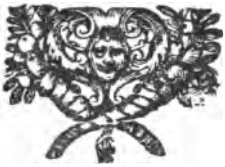
\includegraphics[scale=0.66]{13.livro3_fim.png}
\end{center}
\newpage

%\vspace*{150pt}
\begin{center}
    \vspace*{20pt}
    
\includegraphics[scale=0.33]{12.livro3.png}
\end{center}
\unskip
\vspace{-30pt}
{\let\clearpage\relax \chapter{\Huge LIVRO IV.}}
\unskip
\vspace{-2pt}
\begin{center}
    {\large HISTORIA DA PAYXAM}
\end{center}
\unskip
\begin{center}
    de Chri\lgS to.
\end{center}
\unskip
\par\noindent\rule{\textwidth}{0.4pt}
\unskip\vspace{-3pt}
\section{DIALOGO I.}
\unskip\vspace{-3pt}
\subsection{Proëmial.}
\chaptermark{Dialogo I.}
\sectionmark{Da Oraçãõ de Horto.}

\hspace*{-1.5ex}\begin{minipage}[t]{0.03\linewidth}
    M.\\ \\ \\D.\\ 
\end{minipage}
\hspace*{1ex}\begin{minipage}[t]{1.08\linewidth}
    \lettrine
    [findent =-2pt, nindent=0pt, loversize=-0.2, lraise=0.05, lines=5]
    {\zall{M}}{B}äépe imongaräíbipyra iero-\\
    \hspace*{2ex}biaçábeté, Tupã monhyrõ\\
    \hspace*{2ex}potaçábamo?\\
    Iandé iâra JESUS Chri\lgS to\\
    \hspace*{2ex}rëõagoéra.
\end{minipage}
\begin{alternate}
    \item Maránamopé?
    \item Tupã JESUS Chri\lgS to iandé iâra 
    tecó an-gaipabocáramo cecóreme.
    \item Marã oicôbo pé tecó angaipâba oki?
    \item Omanómo.
    \item Cëõ agoéra recépe Tupã Tûba nhyrõ
    catúramo acêbe?
    \item Cëõagoéra recé.
    \item Ogoemimotáriböépe erímbäé inhëénghi
    ogupïarâma çupé onheranëyma?
    \item Ogoemimotariboé.
    \item Oipotá catú ogoeõ agoéra recé acé\linebreak
    mäendüâra?
    \item Oipotá catú : cecé omäendüáramo é acé
    Tupã rauçubim opyápe ceco abypotarëy-ma.
    \item Marámpe erímbäé cecóu ogoeõ ianondé
    ogoecó auiéramo?
    \item Ombäéú goemimböé etá pyri carúkeme,
    Santi\lgSS imo Sacramento mëénga ianondé.

\end{alternate}

\vspace{2pt}
\par\noindent\rule{\textwidth}{0.4pt}
\unskip\vspace*{2pt}
\section{DIALOGO II.}
\unskip\vspace{-8pt}
\subsection{Oração do Horto.}

\chaptermark{Dialogo II.}
\sectionmark{Da Oração do Horto.}
\vspace*{2pt}

\comecalista{M.}{D.}{M}{A}
    {mópe ixóu ombäéú pábire?\\
    Amó abá remityme.}

\begin{alternate}
    \item Abápe ogueraçó öirúnamo äé mityme?
    \item MOçapyr oboiá, Saõ Pedro, Santiago, Saõ
    Joaõ ceríbäé.
    \item Umámepe amó äé reîâri?
    \item Mitymbïáripe.
    \item Marã ëípe oboiá moçapyr çupé mityme
    oiké riré?
    \item Näétenhé ã tecó teb\~e xe ânga apycyki, ëí:
    iké nhé peicó xerarômo, xepyri pekerëy-
    ma, ëí.
    \item Oieiyipe äé oboiá moçapyr çüí äéreme?
    \item Oieiyi.
    \item Marã oicópotápe?
    \item Ogûba monghetá potá.
    \item Marãpe cêni ogûba monghetâbo?
    \item Oëndypyãëybo ybype oieaybyca.
    \item Marã ëípe oierurêbo?
    \item Tirambúer ã xeremiporarárâma, xe rú-
    bigoé, ëí.
    \item Marã ëí bépe ixupé?
    \item Aipó xe rëõnâmarambuépra abäyme, to-
    nhe monhãnghumé xeremimotâra ëí, nde
    ipotaçâbo catú é, tonhemonhang ëí, ta-
    manône, ëí.
    \item Oür iebype erímbäé oboiá reiaçagoeri-
    pe?
    \item Oúr iebyr.
    \item Marãpe iboiá recóu?
    \item Okér ocoápa recó teb\~e çüí nhé.
    \item Marã ëípe iandé iâra ixupé?
    \item Peçäang iepé coritë\~i nhóte xepyri peke-
    rëyma, ëí, xeretá ã doicöetéi omembêca ;
    xe ânga tene nimarâni, oicöeté te catuâ-
    bo, ëí.\pagebreak
    \item Oçóiebype ogûba monghetâbo ceiánó?
    \item Oçó iebyr oieruréçagoéra recébé oieru-
    rêbono.
    \item Mbobype ixíu imonghetâbo?
    \item Moçapyr.
    \item Ianghecó äí catú cerã iandé iâra imon-
    ghetá pucuábo?
    \item Ianghecó äí catú.
    \item Marã cecó recépe ianghecóäîba iecüâbi?
    \item Cyaîa recé.
    \item Mbäé abyarëymape cyaîa?
    \item Tuguy tikyroéra abyarëyma opiránga-\linebreak
    mo ybype ocyryca.
    \item Döûripe Caräibebé amó ybâca çüí ixu-
    pé oiepiacûca?
    \item Oúr imöapycyca, imotagäípa.
    \item Oúr benhépe oboiá rupâpe ogûba mon-
    ghetá çagoéra çüí?
    \item Oúr benhé, ikêra penhé oguacémamo.
    \item Marã ëípe ixupé?
    \item Aipó xemëéngarâma rûri ; pepüám, tia-
    çó çapépeçobaitiámo, ëí.


\end{alternate}
\newpage

\vspace{2pt}
\par\noindent\rule{\textwidth}{0.4pt}
\unskip\vspace*{2pt}
\section{DIALOGO III.}
%\unskip\vspace{-1pt}
\subsection{Da pri\lgS aõ do Senhor.}

\chaptermark{Dialogo III.}
\sectionmark{Da pri\lgS aõ do Senhor.}
\vspace*{2pt}

\comecalista{M.}{D.}{A}{B}
    {ápe imëéngáramo tûri?\\
    Amó ibóia Judas ceríbäé.
    }

\begin{alternate}
    \item Cetápe Judeos iandpe iâra pycyca cemïe-
    raçopuéra?
    \item Cetá.
    \item Mbäé mbäépe ipópeçoáramo?
    \item Itamímbucú pab~e, itãga pêma, ybyráy-
    çânga, cecäy pyt\~u mimbyca rupi pé re-\linebreak
    çapêbo.
    \item Oicüapámëéng umãpe Judas iandé iâra
    Judeos çupé erímbäé?
    \item Oicüapá meéng umã.
    \item Marã oiâbo pe?
    \item Aéacétobapé pyténe, oiâbo, peipycyc ca-
    tú corí, ipó poá, ixamöína, cecé pemaenã-
    gatuâbo, oiâbo.
    \item Océtobapé pytépe erímbäé cecé ocyca\linebreak
    bé?
    \item Ocetobapépytér, eicobé catú, xe mböe-
    çár guy, oiâbo.
    \item Marã ëípe iandé iâra ixupé?
    \item Mbäé recépe ereiúr, xe remïauçú catú\linebreak
    guy, ëí tëõ çupé xemëéng, xerobápyter\linebreak
    iepé, ëí.
    \item Aépe Judeos çupé marã ëí?
    \item Mbäépe pececar? Eí : nacemïecâra cüa-
    bëyma rüã.
    \item Marã ëípe Judeos?
    \item JESUS Nazareno orocecár, ëí.
    \item Marã ëípe iandé iâra?
    \item Ixé äé ã, ëí.
    \item Marã iabépe Judeos recóu äéreme?
    \item Opá iieäkipué reroiebyri, öatucupê pyté-
    ribo öáybype.
    \item Oporandúbénhépe iandé iâra ixupe abá-
    pe pececár oiâbo?
    \item Oporandúbénhé.
    \item Marã ëípe Judeos ipïaretá ixupé?
    \item JESUS Nazareno icó orocecár, ëí.
    \item Marã ëípe iandé iâra?
    \item Ixé äé ã, äé umã nacó pëêmo, ëí : xe ipó
    xerecárpeiepé : teinhé ã xeboiá omara-\linebreak
    nëyma reraçôbo rëá, ëí.
    \item Marãpe Judeos recóu äéreme?
    \item Opá icyki iandpe iÂra recé, ipopoâbo.
    \item Marãpe iboiá recóu emomã oiâra rere-
    có repiâca?
    \item Saõ Pedro itngapêma ocekyi, morobi-\pagebreak
    \linebreak xába rembïauçûba, Malco ceríbäé apixâ-
    pa inambí mondôca.
    \item Marã ëípe iande iâra ixupé?
    \item Eimondéb itangapêma çurúpe, ëí : nde
    reipotâri pïã xerûba remimotâra rupí xe
    rëõ? Eí.
    \item Oipoçanónghipe iandé iâra äé imambí
    mondokipyra?
    \item Oipoçanóng, inambí ato\~ia nhóte, aunhé-
    nhé imocäémo, imoiepotá.
    \item Marãpe iboiá recóu iandé iâra guá ipó-
    poáreme?
    \item Oiabáb ixüí, ceiá oçôbo, Judeos çüí ocy-
    kyiâbo, omböeçâra reiá.
    

\end{alternate}


\vspace{2pt}
\par\noindent\rule{\textwidth}{0.4pt}
\unskip\vspace*{2pt}
\section{DIALOGO IV.}
%\unskip\vspace{-1pt}
\subsection{Como tratou a Chri\lgS to, Anàs.}

\chaptermark{Dialogo IV.}
\sectionmark{Do que pa\lgSS ou com Anás}
\vspace*{2pt}

\comecalista{M.}{}{M}{A}
    {mópe Judeos iandé iâra reraçóu
    \hspace*{2ex} ipycykire?
    }
\begin{altereven}
    \item Morobixâba Anás ceribäé çupé.
    \item Docoípe iboiá amó cakipoéri?
    \item Oçó Saõ Pedro, Saõ Joaõ abé.
    \item Oiképe äé iboiá äé Anás rokupe?
    \item Oiké.
    \item Marã ëípe cunhã okêna rerecoára Saõ\linebreak
    Pedro çupe?
    \item Có abá boiá räã té picó ndé, ëí. 
    \item Marã ëípe Saõ Pedro?
    \item Näâni, na iboiá rüã ixé? ëí; tëyípe catú
    icüacûpa.
    \item Mbobype aipó ïéu?
    \item Oiepé, Tupã nhëénga abyâbo nhé.
    \item Aé rupíbépe guyrá çapucai?
    \item Çupí bé.
    \item Marã ëípe Anás iandé iâra çupé oporan-
    dûpa?
    \item Umámepe nde boiá etá? ëí. Marã erépa-
    mé oporomböêbo? ëí.
    \item Marã ëípe iandé iâra?
    \item Tëyípe memé nhé ixé popromböé, ëí :
    Marã pipó ixêbo nhé ereporandúb? ëí :
    xe nhëénga renduparoéra çupé eté epo-\linebreak
    randúb, ëí. 
    \item Marã iabépe cerecóu guá äipó ïére-\linebreak mé?
    \item Morobixâba boiá amó oçobápetéc: E-\linebreak
    monãpipó morobixâba erenheéngobai-\linebreak
    xóar? oiâbo.
    \item Marã ëípe iandé iâra ogobápetecaroéra
    çupé?
    \item Emombëú xenhëengäíbagoéra, xe nhë-\pagebreak
    \linebreak éng memoágoéra, ëí:äé çupí catú marã xe
    éreme, marãpe erepóar xe recé? ëí.
\end{altereven}


\vspace{2pt}
\par\noindent\rule{\textwidth}{0.4pt}
\unskip\vspace*{2pt}
\section{DIALOGO V.}
%\unskip\vspace{-1pt}
\subsection{Suce\lgSS o em ca\lgS a de Caiphas.}

\chaptermark{Dialogo V.}
\sectionmark{Suce\lgSS o com Caiphas.}
\vspace*{2pt}

\comecalista{M.}{}{M}{A}
{mópe Anás iandé iâra reraçó
    \hspace*{2ex}ucâri?
    }

\begin{altereven}
    \item Morerecoâra Caiphas ceríbäé çupé.
    \item Marã ëípe Judeos ixupé imonbegoâbo?
    \item Onhëéng monha monháng tenhé o-
        möémamo, ijucáucá potánhé.
    \item Marápe iandé iâra recóu äéreme?
    \item Opic öâma, inhëéng obaxoarëyma.
    \item Marã ëípe Caiphas ixupé oporandûpa?
    \item Tupã eté recé aporandúb endêbo, ëí, ei-
        mombëú catú, Tupã Räyramo nde recó,
        orêbo, ëí.
    \item Marã ëípe iandé iâra ixupé?
    \item Ndé é aipó eré, ëí: anheté, pecepiác irã
        Tupã Tûba ecatüâba coty xe goapyca
        xerêna né, ëí : yby tîngaárybo xe rûra
        abéne, ëí.
    \item Marã ëípe Caiphas Judeos etá çupé, ian-
        dé iâra aipó éreme?
    \item Tupã recé turüã có nhëênga reityki, ëí:
        pecendú nacó inhëênga poxy, ëí. Marã
        etë\~i pipó pëêmo? ëí. Marã ëípe penhëén-
        ga? ëí: öãobuçú mondorondorôca oma-
        ramoráramo.
    \item Marã ëípe Judeos äéreme.
    \item Jajucá memé aipó iâra, ëí: tomanó, ëí.
    \item Marã iabépe maranarí tecoâra cerecóu
        äéreme?
    \item Oixamicyc ceröâma iáiâia, çobá recé \linebreak
        onhenomúnomûna, äôba ib\~i pupé çobá
        ubâna, çobá petépetêca, iaypy atycáty-\linebreak
        câbo : eicüá räú nde ri poparíbäé, oiâbo,
        ixupé.
    \item Opábanhé cerã erimbäé äépe
        tecoára iiaó iaóu, çobá petépetêca?
    \item Opábenhé, pyçaré cerecó memoã bé re-
        rocöêma.
    \item Oiké umã pe Saõ Pedro Caiphas rókupe
        äéreme?
    \item Oiké umã.
    \item Marãpe cecóu?
    \item Tëyípenhé igoapyki, tatá ipype oiepegoá-
        bo
    \item Marãpe ëípe guá ixupe?
    \item JESUS boiá ã icó, ëí.
    \item Mbobype aipó ïéu ixupé?
    \item Moco\~i.
    \item Marã ëípe Saõ Pedro?
    \item Daicüâbi äé abá, ëí, Tupã recé oiâbo te-
        nhé, öemëénamo Tupã rêra réno\~ia.
    \item Oiaby eté catú cerã Tupã nheênga aipó oiâbo?
    \item Oiaby eté catú.
    \item Doicüâbipe aipó roiré öangaipaâba?
    \item Oicüáb, oioëcé iandé iâra mäéneme.
    \item Marã cecó recébépe icüâbi?
    \item Guyrá çapucâia recébé.
    \item Marã iabépe?
    \item Iandé iâra nheéngoéra recébé omäen-\linebreak
        düáramo.
    \item Marã ëípe umã iandé iâra ixupé.
    \item Moçapyr ipó xeboiáramo nde recó erei-
        cüacúb, moco\~i guyrá çapucai ëymebé\linebreak 
        ne, ëí.
    \item Marãpe Saõ Pedro recóu öangaipaba\linebreak
        cüâb ire?
    \item Ocêm ocáripe oiacëõäçycatuâbo.
    \item Aépe Judas noicotebe\~i, Judeos çupé oiâ-
        ra mëengagoêra recé?
    \item Oicó teb\~e.
    \item Marãpe cecóu tecó teb\~e çüí?
    \item Oimëéng ieby cepypoêra morobixâbetá
        ijaroêra çupé, Aiaby eté icó Tupã nhë-\linebreak
        \newpage
        ênga, xe iâra angturameté mëênga, oíâ-\linebreak
        bo.
    \item Marã ëípe Judeos ixupé?
    \item Ndoroicoi aipóbäé recé, ëí: nde ipó\linebreak
        emonã ereicó, ëí: ereicüá ranhé mëêmo
        emonã nde recorâma, ëí.
    \item Marãpe Iudas Recóu äéreme?
    \item Aipó oioupé é abé, oiâra repy poéra rei-
        tyki Tupã rócupé: auié pçôbo oieäiuby-
        ca; ninhyro\~i xoé Tupã ixêbo ne, oiâbo.
    \item Icüábóc cerã moxy oiatimúnga?
    \item Icüapoc.
    \item Opacatú cerã cyghe apüá cúiamo icüá-
        çoro çâba rupí?
    \item Opácátu.
    \item Aépe ïanga, mamópe ixóu?
    \item Anhânga ratápe
    \item Inhyrónhépemo iandé iâra ixupé, Nde
        nhyrõ ixêbo, oioúpe ïéreme mó?
    \item Inhyrõ nhé mó.    

\end{altereven}

\begin{center}
    \vspace*{20pt}
    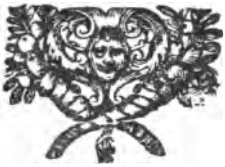
\includegraphics[scale=0.66]{13.livro3_fim.png}
\end{center}

\newpage

\vspace{2pt}
\par\noindent\rule{\textwidth}{0.4pt}
\unskip\vspace*{2pt}
\section{DIALOGO VI.}
%\unskip\vspace{-1pt}
\subsection{Injurias, que recebeo o Senhor nos pa-\\ços de Pilatos, \& Herodes.}

\chaptermark{Dialogo VI.}
\sectionmark{Injurias em ca\lgS a de Herodes.}
\vspace*{2pt}

\comecalista{M.}{}{M}{A}
{mópe erímbäé tëyi catú pab\~e\linebreak
    \hspace*{2ex}iandé iâra reraçou Caiphas rôca\linebreak
    \hspace*{7.8ex}çüí cöemiré?
    }

\begin{altereven}
    \item Pilatos morerecoaruçú çupé, ipó poaçâba
        rebébé ceraçóu.
    \item Marã ëípe ixupé imombegoábo, icoabë-
        ênga?
    \item Nã mbäé ipórbae rüã ocekyi ixupé. Do-
        roguerûrixoémo ndêbo, ïangaipabëyme-
        mo, oiâbo.
    \item Oporandúbpe äéreme Pilatos iandé iâra
        JESUS çupé?
    \item Oporandúb, Iudeos rubixaba pïã ndé,\linebreak
        oiâbo.
    \item Marã ëípe iandé iâra ixupe?
    \item Nde äé aipó eré, ëí.
    \item Marã ëípe Pilatos cerecoaretá çupé?
    \item Naguacém mir\~i angái tecó äíba amó icó
        abá remimonhangoéra, ëí : ïagaipabëy-\linebreak
        ma cüâpa é.
    \item Oieiucá äíbeté cerã ceraçoçaretá äéreme
        opoc\~epocêma?
    \item Oieiucá äíbeté, onhemöaiuábo, inhëénga
        pëpycanhé.
    \item Marã ëípe ?
    \item Oporomöaiú oicôbo, oporomotecócä-\linebreak
        beyma tabá möapaiugoáiugiâbo, Galilea
        çüí catú ïypyrûnga, ëí.
    \item Mamópe Pilatos ceraçóücari äéreme?
    \item Morobixábuçú, Galilea, amó yby, rere-
        côara Herodes ceríbäé çupé.
    \item Çory catú cerã erímbäé Herodes iandé
        iâra JESUS Chri\lgS to repiâca?
    \item Çory catú: coecenhe\~ibé cepiâc potá te-
        nhé roiré.
    \item Maránamo pé çorybamo?
    \item Oimonháng ipó corí milagre amó, mbäé
        ïabäíbäé möabäíbeyma xerobaké ne reá,\linebreak
        oiâbo.
    \item Oimonháng pé iandé iâra amó çobaké?
    \item Noimonhânghi : naxe rerobiá potá rüã 
        moxy recóu xe milagre repiâca potá, oiâ-
        bo.
    \item Oporandúbpe Herodes mbäé tetirüã re-
        cé ixupé?
    \item Oporandúb tenhé: nonheênghi iandé iâ-
        ra ixupé.
    \item Marápe Herodes cerecóücari äéreme?
    \item Doimöetéi; iboiá etá abé irúnamo cere-
        cómemoãmo, äó tînga mondébucá, cecé
        é cerecómemoã çábamo.
    \item Mamópe ceraçóucá iebyri?
    \item Pilatos çupé : äériré oioupé inhyrõ oiere-
        coábamo, coecé nhë\~i oioämotareymiré.
\end{altereven}

\vspace{2pt}
\par\noindent\rule{\textwidth}{0.4pt}
\unskip\vspace{-5pt}
\unskip\vspace*{2pt}
\section{DIALOGO VII.}
\unskip\vspace{-5pt}
\subsection{Dos açoutes do Senhor.}

\chaptermark{Dialogo VII.}
\sectionmark{Dos açoutes do Senhor.}
\vspace*{2pt}

\comecalista{M.}{}{O}{P}
{orandúbé nhépe Pilatos IESUS\linebreak
    \hspace*{2ex}iandé iâra çupé oioupé guá cera-\linebreak
    \hspace*{7ex}çó iebyreme?
}

\begin{altereven}
    \item Oporandúbé nhé, nïangaipâba amó çu-
        pé oguacêma rüã te.
    \item Marã ëítepe Iudeos çupé?
    \item Nagoacém angai ã marã bir\~i icó abá re-
        cópuéra amó çupé, ëí : Herodes mëêmo
        icó oimëéng tëõ çupé, ïangaipâba cüâpa,
        ëí.
    \item Marã ëíbépe ixupe?
    \item Areté goaçú iabiõ ã mundépôramo ïepé
        peimocémucár ixêbo iepí : Peipotápe\linebreak
        JESUS perubixâba ixé imocêma pëémo?
        ëí.
    \item Marãpe Iudeos recóu aipó ïéreme?
    \item Aunhenhé çaceçacémamo, näani, oiâbo,
        doroipotâri ndé imocêma oiâbo, Barra-\linebreak
        bas te eimocém, oiâbo.
    \item Abápe Barrabas?
    \item Abá mondabôra morapitïagoéra repyra-
        mo mundé ócupe imondebipyroéra.
    \item Oimöínibépe Pilatos onhëênga Judeos
        çupé, iandé iâra JESUS mocêma motá?
    \item Oimöínibé moçapyr ixupé onhëênga te-
        nhé; eimoiár, eimoiár ybyrá ioäçâba recé
        imoiâbo nhé, ëí äéreme Judeos, Pilatos\linebreak
        nhëênga rendûpa.
    \item Marãpe Pilatos cerecóucâri äéreme?
    \item Oinupã nupã ucár, toiporëauçúberecó
        Judeos, oiâbo; toicó umé corí ijucäãoâ-\linebreak
        ma recé, oiábo.
    \item Oiaöboc cerã guá icatupe nhé imoingô-
        bo inupãnupã iandondé?
    \item Oiaöbóc, itá okitá recé ipopoá imöâma.
    \item Cetápe inupãnupãçâra?
    \item Cetá : cecé oiopurúpuruâbo ocanëõnëó-
        namo.
    \item Ceté ia catúpe guá imoperéperêbi imöu-
        guy cyryca?
    \item Ceté ia catú.
    \item Yby rupíbépe çuguy cyryki?
    \item Yby rupí bé.\pagebreak
\end{altereven}

\vspace{2pt}
\par\noindent\rule{\textwidth}{0.4pt}
\unskip\vspace*{2pt}
\section{DIALOGO VIII.}
%\unskip\vspace{-1pt}
\subsection{Da coroaçaõ de e\lgS pinhos.}

\chaptermark{Dialogo VIII.}
\sectionmark{Da coroaçaõ de e\lgS pinhos.}
\vspace*{5pt}

\comecalista{M.}{}{M}{A}
{rãpe guá iandé iâra rerecóu inu-\linebreak
    \hspace*{2ex}pãnupã riré?
}

\begin{altereven}
    \item Ogueraçó amó ocuçúpe ceroikeábo, äépe
        maranarí tecóaretá reinhânga recé.
    \item Marã cerecôbo pe?
    \item Iäobôca, amó äópirânga modêpa cecé.
    \item Mbäépe onóng ïacanga áribo?
    \item Iúät\~iembó apynha ïacáng cutúcutûca ça-
        çâpa.
    \item Çuguy cyryc cerã çobá rupí, ïatucupé\linebreak
        rupí bé?
    \item Çuguy cyryc.
    \item Mbäépe oimëéng ïecatüâpe?
    \item Tacoâra, oiepynã ëybo çobaké omemoá-
        namo, imöubixábixábixabäûba.
    \item Marãpe cerecóu äé tacoára mëênghiré?
    \item Onhemunhem\~u çobá recé, ipetépetêca,
        iacánga recé äé tacoára reropoá.
    \item Mamópe Pilatos cenocêmi äéreme?
    \item Ocáripe moröepiacápe Iudeos çupé ce-
        piacucá, imondó nhé motá.
    \pagebreak
    \item Marã etë\~ipe JESUS öenocême?
    \item Aó pirânga, iú abé oguerúr oioëcé oporë-
        auçubeté catúramo.
    \item Marã ëípe Pilatos Iudeos çupé?
    \item Icó abá arúr iké ocáripe cenocÊma tapei-
        cüáb cecó poéra amó ixé cecâra iepé, iju-
        cäucári ianondé guiiâbo, ëí.
    \item Marãpe Iudeos recóu äéreme?
    \item Opoc\~epo\~e opábenhé cecé :  Eimoiarucár
        ybyrá ioáçâba recé, oiâbo : imondó tenhê-
        mo, ndereicói Ce\lgS ar nde rubixâba rauçu-
        páramo, oiâbo.
    \item Oçapiáripé Pilatos inhëênga äéreme\linebreak
        cöyte?
    \item Oçapiár Iudeos çüí ocykyiêbo nhe, xe-
        cüäucámo xerubixâba çupé mo, oiâbo.
    \item Marãpe Pilatos recóu äéreme?
    \item Oiepöéi tëyia remiepiácamo.
    \item Marã oiâbo pe?
    \item Naxeremimotára rupí rüã aiucäucáne,\linebreak
        oiâbo: Naxé recé rüã ijucaçâba árine,\linebreak
        oiâbo.
    \item Marãpe iandé iâra rerecóu äé roiré?
    \item Oimëéng ipópe catú, perecó potaçâbo é
        perecó, ijucâbo, oiâbo.

\end{altereven}
\newpage

\vspace{2pt}
\par\noindent\rule{\textwidth}{0.4pt}
\unskip\vspace*{2pt}
\section{DIALOGO IX.}
%\unskip\vspace{-1pt}
\subsection{Como o Senhor levou a Cruzás co\lgS tas,\\
            \& foi nella crucificado.
}

\chaptermark{Dialogo IX.}
\sectionmark{Da Cruzás costas.}
\vspace*{18pt}

\comecalista{M.}{}{M}{A}
{rãpe Iudeos iandé iâra rerecóu-\linebreak
    \hspace*{2ex}oióupé Pilatos imëénghiré?
}

\begin{altereven}
    \item Ocáripe cenocêmi Cruz nônga iatiybári.
    \item Turuçú catúpe äé Cruz erímbäé?
    \item Turuçú catú : deitëé ceröáröá ceraçôbo
        ipòcyia çüí.
    \item Dogoárucáripe Iudeos äé Cruz abá çupé
        ipytybômo?
    \item Ogoárucár Simão Cireneo ceríbäé çupé.
    \item Iporëauçuberecôbo pe emonã cecóu.
    \item Näâni,tocyc eçapyá,oiucäãoâme oiâbo é.
    \item Doicóipe abá amó, çakipoéri iporëauçu-
        berecóçáramo?
    \item Oçó cunhã cemimböé etá çapirômo.
    \item Marã ëípe iandpe iâra ixupé?
    \item Peteumé xerapirômo, ëí : pë\~e äé eté pe-
        ieapirõ, ëí: pe membyra té peçapirõ, ëí.
    \item Marã oiâbo pé aipó iéu?
    \item Oiucaagoéra repyramo tabuçú Ieru\lgS al\~e,\linebreak
    \newpage
        ipôra recé bé guá imocanhêmäagoáma\linebreak
        cüâpa, aipó oiâbo.
    \item Oçobácype amó cunhã?
    \item Oçóbácyb äótînga pupé, äé recé çobá rä-
        angâbapytáu.
    \item Mamópe guá iandé iâra rerocyki cöyte?
    \item Ybytyra Monte Calvario iápe, äépe imo-
        iá Cruz recé.
    \item Oiaöboc ranhépe guá?
    \item Oiaöbóc.
    \item Oiáratã cerã ïäóba inupãçagoéra imope-
        ré perêbaagoéra recé?
    \item Oiár atã, ndeitëé äéreme Judeos cekyi\linebreak
        atâmo ipîra abé ôca, çuguy mocyryca\linebreak
        ixüí.
    \item Iäógoéra pe marã cerecóu?
    \item Iiucáçarâma oimoiaóc oioupé.
    \item Icatúpenhépe ïâmi tëyipe?
    \item Icatúpe nhé, ixy äé ipó oiaçöí öacânga
        ob\~i pupé.
    \item Marãpe guá cerecóu äé riré?
    \item Oipyçó ybyrá ioäçâba árybo, itá pygoá
        pupé ipó catûca imoiá.
    \item Oguatá iepé cerã ïïybá moco\~i a itá pygoá
        coarâma recé?
    \item Oguatá iepé.
    \item Marãpe guá cerecóu imondyca potá?
    \pagebreak
    \item Opaçáma pupé inhapyt\~io cekycekyi eté-
        bo icanga iepotaçâba pëâbo oió çüí.
    \item Aéramë\~ipe gua ipy rerecóu itá pygoá pu-
        pé imoiáno?
    \item Aéramë\~i.
    \item Aeibépe guá Cruz möâmi iatycâbo?
    \item Aeibé.
    \item Abá abápe oimöámirúnamo amó äé Cruz
        recé?
    \item Moco\~i mondabôra, ïecatüâba coty amó,
        äé amó ïaçú coty.
\end{altereven}

\vspace{2pt}
\par\noindent\rule{\textwidth}{0.4pt}
%\unskip\vspace{-0pt}
\unskip\vspace*{2pt}
\section{DIALOGO X.}
\unskip\vspace{2pt}
\subsection{Do que pa\lgSS ou na Cruz.}

\chaptermark{Dialogo X.}
\sectionmark{Do que pa\lgSS ou na Cruz.}
\vspace*{2pt}

\comecalista{M.}{}{M}{A}
{rã ëípe iandé iâra oiucaçâra ri\linebreak
    \hspace*{2ex}ogûba monghetâbo?
}

\begin{altereven}
    \item Nde nhyrõ ixupé xerubiguy, ëí : oteco-
        cüabëymamo nhé emonã xererecóu, ëí.
    \item Oityc pe guá erímbäé nhëênga cecé?
    \item Oityc, Judeos etá Cruz robâbo, pérupí
        ogoatábäé abé.
    \item Abá abépe nó?
    \item Aipó ipyri imoiâripyroéra abé.
    \item Doimöacyi amó onhëéngäíbagoéra iiaó
        re?
    \item Oimöacy iecatüâba coty ö\~ibäé; deitëé\linebreak
        öapixâra acacâpa cepyca.
    \item Aépe iandé iâra çupé marã ëí?
    \item Nde mäendüár xe recé nde rorypápe nde
        recó roiré, ëí.
    \item Marã ëípe iandé iâra inhëéngobaixóa?
    \item Corí ereicó ce rorypápe xe pyri né, ëí.
    \item Abá abépe öám Cruz ipype äéreme?
    \item Ixy, ianâma Saõ Ioaõ abé, cunhã angatu-
        rámetá abé.
    \item Marã ëí JESUS iandé iâra ocy çupé
        ogoeó ianondé?
    \item Eboqué nde membyra cunhã goé, ëí. Saõ
        Ioão mëênga imembyramo.
    \item Aépe Saõ Ioaõ çupé marã ëí?
    \item Eboqué nde cy, ëí, ixyramo ocy mëénga.
    \item Oimonghetá abépe Päí IESUS ogûba?
    \item Oimonghetá abé, oçapucaîa, ogoacéma-
        mo, maránamo piã xé pea ïepé xerubi-\linebreak
        góe, oiâbo.
    \item Marã ëípe äé riré?
    \item Oguguy embâbagoéra çüí öúcéiamo xe
        úcéi ã, ëí.
    \item Oimöyûpe guá?
    \item Oimöyú.
    \pagebreak
    \item Mbäé pupé pe?
    \item Mbäé pyá upiâra caõ\~i aiácy recé imonãn
        ipupé cëyma.
    \item Marã ëípe çäáng riré?
    \item Auié ã cöyte, ëí.
    \item Marã ëípe ogûba çupé oiekyi ianondé?
    \item Nde pópe catú xe ânga aimëéng xe rubi-
        goé, ëí.
    \item Marãpe cecóu äé roiré?
    \item Oieäybyc ogoacé goacémamo, omanó\linebreak
        catuâbo cöyte.
\end{altereven}

\vspace{15pt}
\par\noindent\rule{\textwidth}{0.4pt}
%\unskip\vspace{-0pt}
\unskip\vspace*{2pt}
\section{DIALOGO XI.}
\unskip\vspace{2pt}
\subsection{Succe\lgSS os depois da Morte de Chri\lgS to.}

\chaptermark{Dialogo XI.}
\sectionmark{Succe\lgSS os depois da Morte.}
\vspace*{10pt}

\comecalista{M.}{D.}{M}{A}
{rãpe tecó iiekyí ianondé?\linebreak
    Coaracy onhemoputun, yby o-\linebreak
    \hspace*{-1ex}bubúr otumú tumûnga,itá oiecáiecá oio-
    \hspace*{-1ex}pyteríbo.
}
\begin{alternate}
    \item Marã ëípe çupiaroéra oçôbo cëõboéra
        reiá?
    \item Tupã Räyreté anhé icó abá, ëí : amó amó
        opotiá recé opoápoá öangaipagoéra möa-
        cyábo.
    \item Abápe opytá äépe?
    \item Ixy, ir~u etpa oiacëó erecôbo öîna.
    \item Obobépe amó abá äépe nó?
    \item Oçóbé amó maránari tecoâra, äé moco\~i
        mondabôra retymá mopena iiucá etêbo,
        ceroiypa abé.
    \item Aépe iandé iâra rëõboéra marã cerecóu?
    \item Itamína pupé iyké catúki, inhyã mobôca,
        aunhénhé y, çuguy abé ixüí i\~emi, ocyryca.
    \item Aépe maranarí tecoára çó riré marã?
    \item Amó moco\~i iandé iâra boiá Jo\lgS eph, Ni-
        codemus abé ceribäé oçó äépe.
    \item Mbäé recépe ixóu?
    \item Cëõboéra reroiypa, itymamotá.
    \item Marãpe cerecóu itymi iandondé?
    \item Aó tînga pupé inhubâni, itá caramemoã
        abátymagoerëyma pupé imondêpa.
    \item Abã abépe ipyri itymbáramo?
    \item Ixy, ir\~u etá abé.
    \item Marãpe cecóu ipupé iondêbiré, ixüí\linebreak
        oçôbo?
    \item Oçokendáb äé itá caramemoã guaçú pu-
        pé.
    \item Oiacëó erecó abé cerã ogoeraçó ogócu-
        pe?  
    \item Oiacëé erecó abé. Päí JESUS recobé ie-
        byraõama recé onhemiçacuîâbo.

\end{alternate}

%\vspace*{150pt}

\begin{center}
    \vspace*{20pt}
    
\includegraphics[scale=0.40]{12.livro3.png}
\end{center}
\unskip
\vspace{-30pt}
{\let\clearpage\relax \chapter{\Huge LIVRO V.}}
\unskip
\vspace{-2pt}
\begin{center}
    {\large CATECISMO}
\end{center}
\unskip
\unskip\vspace{25pt}
\begin{center}
    E explicaçaõ dos Mandamentos\\
    da Ley de Deos , \& da Santa\\
    Madre Igreja.
\end{center}
\unskip\vspace{25pt}
\par\noindent\rule{\textwidth}{0.4pt}
\unskip\vspace{-3pt}
\section{DIALOGO I.}
\unskip\vspace{-3pt}
\subsection{Do primeiro Mandamento da Ley\\
de Deos.}
\chaptermark{Dialogo I.}
\sectionmark{Honrarás hum \lgS ó Deos.
}

\hspace*{-1.5ex}\begin{minipage}[t]{0.03\linewidth}
    M.\\ \\D.\\M.\\ 
\end{minipage}
\hspace*{1ex}\begin{minipage}[t]{1.08\linewidth}
    \lettrine
    [findent =-2pt, nindent=0pt, loversize=-0.2, lraise=0.05, lines=5]
    {\zall{A}}{C}erecómonháng pe Tupã\\
    \hspace*{2ex}erímbäé?\\
    Acerecómonháng.\\
    Mbäérâma recépe acerecó-\\
    \hspace*{2ex}monhânghi?
\end{minipage}

\begin{altereven}
    \item Acé ogoapiâra potá.
    \item Maránamope acé çapiárine?
    \item Oiáretéramo cecóreme.
    \item Marãpe Tupã imopoçâra rerecóu ne?
    \item Ybákype ceraçóune.
    \item Aépe ïiabyára?
    \item Anhânga ratápe ceitykine.
    \item Mbobype äé acerecomonhangâba.
    \item Moco\~i acé pó papaçâa rupí ixyki.
    \item Marã ëípe ïypy?
    \item Eimöeté oiépé Tupã, ëí.
    \item Marã oicôbo bépe?
    \item Tupã eté oiepébäé möetêbo, inhëênga\linebreak
        rupí oicôbo.
    \item Marã oicôbo bépe?
    \item Tupã recé oierobiá, äé ipó quépe marate-
        córeme acé porauçubôki, oiâbo.
    \item Marã oicôbo bépe?
    \item Ixupé ogoecoteb\~eçâba recé oierurêbo,\linebreak
        äé äé cóbäé catú mëengâra, oiâbo.
    \item Oçauçu catúpe acé Tupa, imöeté potá?
    \item Oçauçú catú.
    \item Maránamopo acé çauçúbi?
    \item Ogubétéramo, omonhangáramo, opycy-
        roánamo cecóreme.
    \item Marã ëípe acé opyápe Tupã rauçúpa\linebreak
        imöetébo?
    \item Tupã reçápe ã xe recóu, ëí, taicó umé\linebreak
    \newpage
        mbäé poxy recé çobaké cá, ëí.
    \item Abápe aipó Tupã nhëénga oimomarán?
    \item Tupã nhëênga morõböeçâra coty, anhe
        raúpe ëíbäé.
    \item Abá bépe?
    \item Tupã omonhángareté möeteçarëyma,\linebreak
        ixüí catú mbäé amó rerecôbo otupána-\linebreak
        mo imöeté äúba.
    \item Abá bépe Tupã noimöetéi?
    \item Imbäé cüá möangäúbäé aröanëym, Tupã
        recómombegoâra.
    \item Iangaipábetépe abá onhemopaiépaiêbo,
        oporomõgaräíbäúpa anhânga omböeçâ-\linebreak
        ba rupi?
    \item Iangaipábëté.
    \item Abábépe aipó Tupã nhëênga oiaby?
    \item Paié rerobiaçâra.
    \item Marã oicôbo pe abá cerobiári?
    \item Ixupé mbäé amó mëénga, oietanónga,\linebreak
        maranëymiiáramo cecó möangäúpa.
    \item Paié äûba çupé onhemotimbotimboru-
        cáribäé, coipó öäyra, coipó amó abá oixu-
        bánucáribäé abêpe?
    \item Aé abé.
    \item Abé abé aipóbäe oiaby?
    \item Erímbäé ogoamyia recópoêra purúby-\linebreak
        te çáribaé, guyrá, coipó iagoára nhëênga\linebreak
        \newpage
        çupé maranghigoána oiâbo.
    \item Marã oicôbo bépe?
    \item Pitânga nhemonhânga çüí oiepoçanó-\linebreak
        çanônga.
    \item Abábépe oiâby?
    \item Moçauçûba rerobiaçâra, ipór irã ne ïâra.
    \item Abá abépe?
    \item Maratecorâma recé paié monghetaçâra:
        moraceîa, maracá poraceîa rerobiaçâra\linebreak
        abé.
    \item Oiaby bépe aipó, öemirecó membyrâra
        recé oiecüacúbäé, coipó öäyra maräâra\linebreak
        recé, coipó öaiyra nhemondïâra recé?
    \item Oiaby bé.
    \item Paié rerobiaraõâma recé abá mborypâra
        marã pe?
    \item Aé abé oiâby.
    \item Oiaby etépe abá, öúr temó anhânga xe-
        reraçôbo mã, ïâra?
    \item Oiaby eté, opyá catú çüí aipó oiâbo é.    
\end{altereven}

\begin{center}
    \vspace*{20pt}
    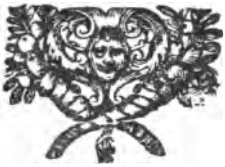
\includegraphics[scale=0.50]{14.livro3_dialogo2.png}
\end{center}

%\newpage
\vspace{2pt}
\par\noindent\rule{\textwidth}{0.4pt}
\unskip\vspace*{2pt}
\section{DIALOGO II.}
%\unskip\vspace{-1pt}
\subsection{Do \lgS egundo Mandamento da Ley\\
            de Deos.
}

\chaptermark{Dialogo II.}
\sectionmark{Não tomarás o nome de Deus em vão.}
\vspace*{9pt}

\comecalista{M.}{}{M}{A}
{rãpe ëípe amó äé Tupã acé reco-\linebreak
    \hspace*{2ex}monhangâba?
}

\begin{altereven}
    \item Anheté eré tenhé umé Tupã rêra renô\~ia,
        ëí.
    \item Abápe aipóbäé oiaby?
    \item Iporëymbäé, coipó öemingöá catúëyma
        oimombëúbäé, emonã cõ Tupã recé oiâ-
        bo tenhé.
    \item Oânga, coipó abá ânga, coipó Santo amó
        ybâkype tecoâra reno\~indâra abé oiurára-
        goáiamo nhé, marã pe?
    \item Aé abé oiaby.
    \item Aépe cupindoárëyma recé Cruz reno\~i-
        dâra marã?
    \item Oiaby abé.
    \item Mbäé mir\~i recé tirüã pe aipó oiâbo, Tu-
        pã nhëênga abyetéo?
    \item Mbäé mir\~i recé titüã.
    \item Abábépe oiâby?
    \item Tecó memoã monhangäaõâma recê Tu-\pagebreak
    \newpage
        pã rêra rení\~ibäé, emonã aicóne oiâbo.
    \item Maránemetépe abá, anheté Tupã recé,
        coipó mbäé amó recé ïeú çupi catú?
    \item Imarã gatú çupi é imombëúpyra recóre-
        me é, mbäé catúramo cecóreme é.
    \item Oiaby bépe abá, mbäé catú Tupã recé
        öemïeno\~igoéra moporëyma?
    \item Oiabybé.
    \item Mbäé catú monhangaoáma recé Tupã
        reno\~idâra, näimopó potá rüã, marã pe?
    \item Oiaby bé.
    \item Marã ëí nhóte tépé acé mbäé mombe-
        goâbo?
    \item Anhé, Anhetê, ëí nhóte.
\end{altereven}

\vspace{15pt}
\par\noindent\rule{\textwidth}{0.4pt}
%\unskip\vspace{-0pt}
\unskip\vspace*{2pt}
\section{DIALOGO III.}
\unskip\vspace{2pt}
\subsection{Do terceiro Mandamento da Ley \\de Deos.}

\chaptermark{Dialogo III.}
\sectionmark{Naõ juraràs, \&c.}
\vspace*{10pt}

\comecalista{M.}{D.}{M}{A}
{rã ëípe amó äé?\\
    \hspace*{-0.2ex}Eimöetê Domingo,âra marãtecoa-
    \hspace*{8ex}bëyma abé, ëî.
}
\begin{alternate}
    \item Abépe aipôbäé oimopòr catú?
    \item Areté pupé Tupã monghetaçâra, Tupã\pagebreak
    \newpage
        recé onhëangherecóçâra oporabykyëy-\linebreak
        ma
    \item Abá bépe oimopór?
    \item Tupáneme Tupã omonhangagoéra recé,
        oió ecé cëõägoéra recé onhëangherecó-\linebreak
        bäé tecó catú recé, Tupã oimoiecoçuba-\linebreak
        goâma recé ixupé oierurêbo.
    \item Abápe aipobäé oiaby.
    \item Domingo pupé, âra marãtecoabëyma pu-
        pé bé oporabykybäé.
    \item Oiaby bépe abá ogoembïauçûba, coipó
        oäyra, coipó öembirecó moporabykyábo?
    \item Oiaby bé.
    \item Mbäé mir\~i monhânga tirüãpe acé ïabyú?
    \item Näâni.
    \item Aépe öapixâra aretéreme oporabykypo-
        táribäé mborupâra, marã?
    \item Aipóbäé abé oiaby.
\end{alternate}

\vspace{2pt}
\par\noindent\rule{\textwidth}{0.4pt}
%\unskip\vspace{-0pt}
\unskip\vspace*{2pt}
\section{DIALOGO IV.}
\unskip\vspace{2pt}
\subsection{Do quarto Mandamento da Ley \\de Deos.}

\chaptermark{Dialogo IV.}
\sectionmark{Honrarás a teu pay, \&c.}
\vspace*{10pt}

\comecalista{M.}{}{M}{A}
{rã ëípe amó äé acé recomonhan-\\
    \hspace*{2ex}gâba?
}

\begin{altereven}
    \item Eimöeté nde rûba, nde cy abé, ëí.
    \item Marã oicôbo pé acé aipóbäé mopôri?
    \item Ogûba, ocy abê moetêbo, inhëênga mo-
        pôra cecoteb\~eçâba rí imoiecoçôpa.
    \item Oçapiárpe abá ogûba, ocy tecómemoã
        amõ recé opoâime ne?
    \item Doçapiarixoéne.
    \item Ogûba anhópe abá oçapiá, aipóbäé mo-
        pô potá?
    \item Ná ogûba anhó rüã, ogubixâba abé tâ-
        ba rerecoâra acé oçapiá.
    \item Abá abépéne?
    \item Cunhã omêna nhëênga rapiá ogûba, ocy
        çórene.
    \item Marã oicôbo pé acé rûba aipó Tupã nhë-
        ênga abyú?
    \item Oäyra recé onheanghecóëymamo, tecó
        catú recé imböéeymamo, imonhemom-\linebreak
        beüucareymamo bé.
    \item Marã oicôbo bépe?
    \item Oäyra marã mir\~i cecóreme, coipó Tupã
        nhëênga abyreme, cenonheneyma, cói-\linebreak
        pó ïaguaçá repiakínamo.
    \item Aépe mïauçûba noçapiaririxóe oiâra\linebreak
        nheênga ne?
    \item Oçapiáne.
    \item iaby bépe iiâra aipó Tupã nheênga ce-\linebreak
    \newpage
        có caturâma recé onhemoçainaneyma?
    \item Oiaby.
    \item Abá bépe acé oçapiáne?
    \item Abaré acé ânga rûba, acé ânga recó catú
        râma recé marã ïéreme.
    \item Abá abépe moetêbo acé aipó Tupã nhe-
        ênga mopone?
    \item Oguekeyra, oenotaroéra, tunhabä\~e abé.
\end{altereven}

\vspace{2pt}
\par\noindent\rule{\textwidth}{0.4pt}
%\unskip\vspace{-0pt}
\unskip\vspace*{2pt}
\section{DIALOGO V.}
\unskip\vspace{2pt}
\subsection{Do quinto Mandamento da Ley \\de Deos.}

\chaptermark{Dialogo V.}
\sectionmark{Não matarás.}
\vspace*{10pt}

\comecalista{M.}{D.}{M}{A}
{rã ëípe amó äé?\\
 Eporapiti umé, ëí.
}

\begin{alternate}
    \item Abápe aipóbäé oimopór?
    \item Opyápe tirüã oapixâra recé marã oecóa-
        goéra recé oiepyc potarëymbäé.
    \item Abápe aipóbäé oiaby?
    \item Abá iucaçÂra, aiucá temó mã ëíbäé abé.
    \item Omanó temo mã, coipó ïiámburú oma-
        nômo, ïiámburú ombäéacyramo, ëíbäé
        abépe?
    \item Aé abé.
    \item Guariniâme oporapitíbäé tirüã pe?
    \item Näâni, ogubixâba nhëênga rupí emonã
        oicôbo é, marâna çupí catú ndoáramo ce-
        córeme é.
    \item Marã oicôbo bépe abá ïabyú?
    \item Oporoapixâpa, oporoyrõramo, oporonu-
        pãnúpâmo.
    \item Doinupãxoé tepe abá oäyra, oemiauçú-
        bane?
    \item Oinupã tecó catú abyagoéra iá nhóte, ce-
        có catú potar é né.
    \item Abá bépe oiaby?
    \item Oiememby iucábäé, oiemembyrakirá ri-
        bäé abé.
    \item Abá abépe?
    \item Opurüá iucá potá moçanghigoâba guâ-
        ra.
    \item Oporúbäé pé marã?
    \item Oiaby eté catú Tupã nhëênga.
    \item Ogoerecómemoãçâra recé oiepyca ti-\linebreak
        rüãpe abá Tupã nhëênga abyú?
    \item Cecé oiepyca tirüã: inhyrõ nhé acé ixupé
        Tupã recéne?
    \item Deitëé cerã acé Tupã monghetaçâpe,\linebreak
        Nde nhyrõn oré angaipâba recé orêbe, oré
        rerecómemoãçâra çupé oré nhyrõ iabé,\linebreak
        oiâbo Tupã çupé?
    \item Deitëé.
    \item Abá bépe oiaby?
    \item Oemiamotarëyma recoâpe oçopotarëy-
        mbäé cepiâca çüí.
    \item Oiaby bépe abá aipó Tupã nhëênga,\linebreak
        opyápe catú oapixâra çupé anhânga, coi-
        pó tëõ, coipó iurûparí rekyîa?
    \item Oiaby bé.
    \item Marã oicôbo bépe abá iabyú?
    \item Cunhã ipurüábäé recé opoá pitânga iu-
        câbo ixüí, coipó iiucá potá.
    \item Marã oicôbo bépe?
    \item Abá rëõ agoéra recé ogorybamo, coipó
        abá cerecómemoã agoéra recé, iiá, oiâbo.
    \item Marã oicôbo bépe?
    \item Tereiucá ixêbo paié äíba çupé oiâbo bé.
\end{alternate}

\vspace{2pt}
\par\noindent\rule{\textwidth}{0.4pt}
%\unskip\vspace{-0pt}
\unskip\vspace*{2pt}
\section{DIALOGO VI.}
\unskip\vspace{2pt}
\subsection{Do \lgS exto, \& nono Mandamento da\\Ley de Deos.}

\chaptermark{Dialogo VI.}
\sectionmark{Não fornicaràs,\&c.}
\vspace*{6pt}

\comecalista{M.}{D.}{M}{A}
{rã ëípe amó äé?\\
 Eporopotárume, ëí.
}

\begin{alternate}
    \item Abápe aipóbäé oiaby.
    \item Iägoaçábäé, omenfaçabëyma recé oicó-
        bäé abé.
    \item Cunhã potá nhóte tirüãpe abá Tupã\linebreak
        nhëênga abyú?
    \item Ipotá nhóte tirüã : cecé opocôca abé,\linebreak
        ïaiubâna, opyá poxyramo cecé iiucáäíba,
        çakipoemendôdo.
    \item Marã oicôbo bépe?
    \item Ixupé onhëênga cecé oicópotá, ixupé oie-
        piácucá, taxé potá oiâbo.
    \item Abá bépe oiaby?
    \item Manhána, cunhã mëêngâra, coipó abá
        çupé imonghetaçâra, coipó imborypâra.
    \item Oiaby bépe abá aipóbäé poxy recé onhë-
        angherecoçâpe, cecé omäendüaçape im-
        borypa?
    \item Oiaby bé.
    \item Marã oicôbo bépe abpa ïabyú?
    \item Mbäé poxy recé opoçauçúbagoéra mo-
        rypa, icatúpe nhé temomã, oiâbo.
    \item Marã oicôbo bépe?
    \item Oiemongatyrômo, abá opotára potá, coi-
        pó xeporángheté temomã, äémo abá xe-
        potari oiâbo bé.
    \item Marã oicôbo bé?
    \item Mbäé poxy coty onhëéngäíbamo, coipó
        ogocupé iopotâra repiak\~iämo.
    \item Taicóne nde recé, oiurúpe nhóte abá çu-
        pé oiâbo bépe, abá aipó Tupã nhëênga\linebreak
        abyú?
    \item Oiurúpe nhóte aipó oiâbo bé.
    \item Abá bépe oiaby?
    \item Ceçá poropotáríbäé, aipotár eté coé cu-
        nhã mã ëíbäé.
    \item Mbobype abá aipóbäé oiaby, cunhã recé
        onhemomotáriré, coipó imonghetá roiré,
        cecé obykëymapucúi?
    \item Cecé omäendära iabiõ, imorambuerëy-
        ma é.
    \item Oiabu etépe aipóbäé cunhãtä\~i ruguyca-
        çâra?
    \item Oiaby eté.
    \item Aépe öanameté recé oicópoxybäé?
    \item Oiaby eté bé.
    \item Oiaby etépe abá Tupã nhëênga onhe-\linebreak
        mombegoápe, goemimomoxypuéra öa-\linebreak
        nametéramo cecó cüacûpa?
    \item Oiaby eté.
    \item Aépe omêna, coipó goemirecó anameté-
        ramo cecó mombëúëyma, marã?
    \item Oiaby eté bé.
    \item Oiaby etépe abá öatüaçâba recé oicôbo?
    \item Oiaby eté té.
    \item Oiaby eté bépe abá Tupã nhëênga oma-
        nhánamo abá moingôbo?
    \item Oiaby eté bé.
    \item Abá bépe?
    \item Opupúcbäé, coipó okêra pupé opupucoé-
        ra mborypa, icatúpenhé temomã, opaca-
        goéripe ëíbäé.
    \item Marã oicôbo bépe abá aipó Tupã nhë-
        ênga abyú?
    \item Cunhã, coipó abá reté recé omäêmo, coi-
        po ogoeté recé mäêmo bé, cecé bé opocô-
        ca oporopotáramo.
    \item Marã oicobo bépe?
    \item Oängaipâba mombegoábo, cecé ogory-
        bamo, coipó onhëêngäíbamo, coipó onhë-
        ênga paparäíbamo.
    \item Oiaby eté bépe cunhã Tupã nhëênga\linebreak
        omêna manhánamo oicôbo, coipó ixupé
        öapixâra amó mëênga?
    \item Oiaby eté bé.
    \item Aépe öagoaçã recé ceguyrómbäé marã?
    \item Oiaby bé.
    \item Oiaby eté catúpe abá Tupã nhëênga öa-
        pixâra robaké, coipó cemïandúbamo cu-
        nhã recé oicôbo?
    \item Oiaby eté catú.
\end{alternate}

\newpage
\vspace{2pt}
\par\noindent\rule{\textwidth}{0.4pt}
\unskip\vspace*{2pt}
\section{DIALOGO VII.}
%\unskip\vspace{-1pt}
\subsection{Do \lgS etimo, \& decimo Mandamento 
    \\da Ley de Deos.
}

\chaptermark{Dialogo VII.}
\sectionmark{Naõ furtarás, \&c}
\vspace*{9pt}

\comecalista{M.}{D.}{M}{A}
{rãpe ëípe amó äé?\\
    Emondarõ umé ëí.
}

\begin{alternate}
    \item Abápe aipóbäé oiaby?
    \item Abá mbäé recé omondarõbäé; abá mbäé
        Om\~ibäé.
    \item Abá abépe?
    \item Abá mondarõagoéra öúbäé, coipó ogócu-
        pe ogoeraçóbäé.
    \item Abá abépe?
    \item Oimomondarõbäé abé: abá mbäé recé
        abá mondarõ ocepiakíbäé: mondarõ re-
        cébé abá pytybômo.
    \item Marã oicôbo bé abá ïabyú?
    \item Abá mbäé mombucâpa, abá rymbâba iu-
        câbo, abá mundéçûpa ipórôca.
    \item Abábépe oiaby?
    \item Oapixâra rymbâba iagoâra remimomo-
        c\~egoéra, coipó cemijucá poéra raçâra.
    \item Abábépe oiabyu?
    \item Marã tecó repyramo, coió mbäé repy-\linebreak
        ramo oemiiaroéra repymondycarëyma.
    \item Marã oicôbo bépe.
    \item Mbäé canhêma ogoacémaagoéra ïjâra\linebreak
        çupé imëénghëyma.
    \item Marã gatúpe abá recóu omondarõ recé
        oioupé Tupã nhyrõ motá?
    \item Ogoeroieby, coipó oimöepy omondaça-
        goéra.
    \item Oiaby bépe abá Tupã nhëênga abá mbäé
        recé onhemomotá, anhom\~i temó imbäé
        catú mã, oiâbo?
    \item Oiaby eté, Enhemomotárumé abá mbäé
        recé, Tupã acerecomonhangápe, ïéreme.
    \item Marã oicôbo bépe acé aipó Tupã nhë-
        ênga abyú?
    \item Abá mbäé catû rerecó moacyâbo, n\~ibäé
        catúi xoétemó ah\~e mã, oiâbo.
\end{alternate}

\vspace{2pt}
\par\noindent\rule{\textwidth}{0.4pt}
%\unskip\vspace{-0pt}
\unskip\vspace*{2pt}
\section{DIALOGO VIII.}
\unskip\vspace{2pt}
\subsection{Do oitavo Mandamento da Ley\\de Deos.}

\chaptermark{Dialogo VIII.}
\sectionmark{Não levantarás fal\lgS o te\lgS tem.}
\vspace*{6pt}

\comecalista{M.}{D.}{M}{A}
{rã ëípe amó äé?\\
 Nde remöemumé abé recé, ëí.
}
\begin{alternate}
    \item Abápe aipóbäé oiaby?
    \item Abá recé möéma monhangâra.
    \item Marãpe abá recóu oapixâra recé oemö-
        em iré, oióupé Tupã nhirõ mota?
    \item Xeremöém aipó guiiábo, ëí, ogoendupâ-
        rêra çupé onhëênga recobiarômo.
    \item Marã oicôbo bépe abá aipóbäé abyú?
    \item Abá angaipanhemîma icüaparëyma çu-
        pé mombegoábo?
    \item Deicatú angáitepe acé abá recó nhemî-
        ma mombegoábo?
    \item Eicatu ipó cenonhendarâma çupé é, imo-
        ingó catúçarâma çupé é.
    \item Aepe onhemombegoápe cemöembäé,\linebreak
        marã?
    \item Oiaby etété catú nhé oangaipagoéra cüa-
        cûpa, coipó oangaipâba möânga.
    \item Oiaby bépe abá Tupã nhëênga onhemõ-
        begoápe tirüã abaré çupé abá ïangaipá-\linebreak
        bäé rêra mombegoábo?
    \item Oiaby bé.
    \item Marã oicôbo bépe ïabyú?
    \item Abá marã éagoéra mombegiábo, ómbäé
        poéramo, abá recé nhöamotarëyma rere-
        cóucá abá çupé.
    \item Marã oicóbo bépe?
    \item Cunhã cüäucá  imêna çupé, emonã racó
        cecóu nde çüí, oiâbo.
\end{alternate}

\end{document}


